% 内积空间（内积与诱导范数、Gram矩阵）、正交与投影（正交补、标准正交基、Gram--Schmidt正交化、正交投影）、线性泛函的内积表示与伴随。

\section{内积空间}
\label{sec:ls-inner-product-spaces}

范数只度量大小，不给出角度。一般范数下谈不上两个方向是否垂直，向子空间的最近点也可能不唯一（示例~\ref{ex:ls-linf-nonunique-nearest}）。第~\ref{chap:linear-operations}章在$\mathbb R^d$上用逐项相乘再求和定义了欧氏内积，并由它得到长度和夹角。本节提取这种计算的共同规则，在一般线性空间上定义内积。

本节先从内积公理推出长度、夹角和几个基本不等式，再用Gram矩阵记录一组向量的两两内积。正交投影、标准正交基和伴随在随后两节讨论。

\subsection{内积与内积诱导的范数}
\label{sec:ls-inner-product-definition}

本小节先给出内积的公理和例子，再由内积定义长度、正交与夹角，最后从三角不等式出发，说明内积诱导的长度是范数，从而给出距离；平行四边形恒等式则说明，并非每个范数都来自内积。

\subsubsection{内积的定义}
\label{sec:ls-inner-product-axioms}

欧氏内积对每个变量都保持线性组合，交换两个变量不改变结果，向量与自身的内积只在零向量处为零。这些性质只涉及线性运算，因此可以用来定义一般空间上的内积。
\begin{definition}[内积空间]
\label{def:functional-inner-product-space}
\label{def:linear-algebra-inner-product}
设$V$是实线性空间。映射$\langle\cdot,\cdot\rangle:V\times V\to\mathbb R$若对任意$\bm x,\bm y,\bm z\in V$与$a,b\in\mathbb R$满足
\begin{enumerate}
 \item 双线性：$\langle a\bm x+b\bm y,\bm z\rangle=a\langle\bm x,\bm z\rangle+b\langle\bm y,\bm z\rangle$，且$\langle\bm z,a\bm x+b\bm y\rangle=a\langle\bm z,\bm x\rangle+b\langle\bm z,\bm y\rangle$；
 \item 对称性：$\langle\bm x,\bm y\rangle=\langle\bm y,\bm x\rangle$；
 \item 正定性：$\langle\bm x,\bm x\rangle\geq0$，且$\langle\bm x,\bm x\rangle=0$当且仅当$\bm x=\bm0$，
\end{enumerate}
就称为$V$上的\term{内积}（inner product）；配备内积的线性空间$(V,\langle\cdot,\cdot\rangle)$称为\term{内积空间}（inner-product space）。
\end{definition}

\paragraph{内积的例子}
先检验欧氏内积满足这三条公理。设$\bm x,\bm y,\bm z\in\mathbb R^d$，$a,b\in\mathbb R$。对称性成立，因为每一项$x_jy_j=y_jx_j$。对第一个变量的线性来自有限和的运算法则：
\[
 \sum_j(ax_j+bz_j)y_j=a\sum_jx_jy_j+b\sum_jz_jy_j,
\]
再由对称性，对第二个变量同样成立。正定性成立，因为$\langle\bm x,\bm x\rangle=\sum_jx_j^2\geq0$，而非负数之和为零时每一项都为零。

同形矩阵上的Frobenius内积也满足三条公理。它对两个变量分别线性；交换两个矩阵不改变各项乘积，因而对称；$\langle\bm A,\bm A\rangle_{\mathrm F}=\sum_{i,j}a_{i,j}^2$非负，并且只在$\bm A=\bm0$时为零。这正是把$mn$个元素看作坐标时欧氏内积的三条性质。所以下面从公理推出的一般结论对它同样成立。

标准内积之外，一般空间上还可以有各种内积。下面在$P_1$上规定一个只看两点取值的内积，后面的算例会反复用到它。
\begin{example}[只看两点取值的内积]
\label{ex:ls-two-point-inner-product}
给定：$P_1$上的规则$\langle f,g\rangle=f(0)g(0)+f(1)g(1)$。

验证：右端对$f$与对$g$分别是线性的，交换$f,g$也不改变右端，所以双线性与对称性成立。$\langle f,f\rangle=f(0)^2+f(1)^2\geq0$；若它为零，则$f(0)=f(1)=0$，对$f=a+bt$即$a=0$、$a+b=0$，故$f=0$，正定性也成立。

结论：这一规则是$P_1$上的内积。它只看函数在$t=0,1$两点的取值，与系数向量$(a,b)^\top$的欧氏内积不同：例如$\langle1,t\rangle=1\cdot0+1\cdot1=1$，而$1$与$t$的系数向量$(1,0)^\top$、$(0,1)^\top$的欧氏内积为零。
\end{example}

\paragraph{复内积的约定}
上面的定义针对实空间。在复空间中，若两个变量都按复数线性，并且满足实数式的对称性，那么$\langle\mathrm i\bm x,\mathrm i\bm x\rangle=-\langle\bm x,\bm x\rangle$，无法对非零向量保持正定。因此复内积采用另一种约定：对第一个变量共轭线性，对第二个变量线性，并满足$\langle\bm x,\bm y\rangle=\overline{\langle\bm y,\bm x\rangle}$。标准例子是$\langle\bm x,\bm y\rangle=\bm x^*\bm y$，其中$\bm x^*$表示共轭转置；仍要求$\langle\bm x,\bm x\rangle>0$对非零$\bm x$成立。

后面的Cauchy--Schwarz不等式在复内积下同样成立。若$\bm y\ne\bm0$，在$\lVert\bm x-\alpha\bm y\rVert^2\geq0$中取$\alpha=\langle\bm y,\bm x\rangle/\lVert\bm y\rVert^2$，展开可得$|\langle\bm x,\bm y\rangle|^2\leq\lVert\bm x\rVert^2\lVert\bm y\rVert^2$。因此它的平方根仍给出范数。但复内积的值可能不是实数，下一小节用余弦定义夹角的公式不能直接照搬。下文的证明继续使用实内积，复情形需要把转置相应改为共轭转置。

\subsubsection{由内积定义的夹角}
\label{sec:ls-inner-product-angle}

\paragraph{长度与正交}
与$\mathbb R^d$中一样，内积给出长度$\lVert\bm v\rVert=\sqrt{\langle\bm v,\bm v\rangle}$，它是否满足范数的全部要求，留到下一小节检验；$\langle\bm x,\bm y\rangle=0$时称$\bm x,\bm y$正交。正交的两个向量满足勾股定理。展开
\[
 \lVert\bm x+\bm y\rVert^2=\lVert\bm x\rVert^2+2\langle\bm x,\bm y\rangle+\lVert\bm y\rVert^2,
\]
交叉项为零，得$\lVert\bm x+\bm y\rVert^2=\lVert\bm x\rVert^2+\lVert\bm y\rVert^2$。

\paragraph{Cauchy--Schwarz不等式}
平面上两个非零向量的夹角$\theta$满足
\[
 \langle\bm x,\bm y\rangle=\lVert\bm x\rVert\,\lVert\bm y\rVert\cos\theta.
\]
要在一般内积空间中反过来用这个关系定义夹角，须先保证内积除以两个长度之积后总落在$[-1,1]$中。下面的不等式给出这一保证。
\begin{theorem}[Cauchy--Schwarz不等式]
\label{thm:linear-algebra-cauchy-schwarz}
对任一内积及其长度，任意向量$\bm x,\bm y$满足
\begin{equation}
 |\langle\bm x,\bm y\rangle|\leq\lVert\bm x\rVert\,\lVert\bm y\rVert,
 \label{eq:prelim-cauchy-schwarz}
\end{equation}
等号成立当且仅当其中一个向量是另一个向量的实数倍。
\end{theorem}
\begin{proof}
$\bm y=\bm0$时两边都为零。设$\bm y\neq\bm0$。对任意实数$s$，向量$\bm x-s\bm y$的长度平方非负；按内积的对称性与双线性展开，
\[
 0\leq\lVert\bm x-s\bm y\rVert^2
 =\lVert\bm x\rVert^2-2s\langle\bm x,\bm y\rangle+s^2\lVert\bm y\rVert^2.
\]
右侧是$s$的二次函数，二次项系数为正，在顶点$s=\langle\bm x,\bm y\rangle/\lVert\bm y\rVert^2$处最小，最小值为$\lVert\bm x\rVert^2-\langle\bm x,\bm y\rangle^2/\lVert\bm y\rVert^2$。它非负，两边乘以$\lVert\bm y\rVert^2$再开平方，即得不等式。等号成立当且仅当对这个$s$有$\bm x-s\bm y=\bm0$，即$\bm x$是$\bm y$的实数倍；连同$\bm y=\bm0$的情形，即得等号条件。
\end{proof}
证明只用了内积的三条公理，所以不等式对每一种内积都成立。在$\mathbb R^d$的标准内积下，它就是$p=q=2$的Hölder不等式（定理~\ref{thm:linear-algebra-holder}）；对Frobenius内积，它给出$|\langle\bm A,\bm B\rangle_{\mathrm F}|\leq\lVert\bm A\rVert_{\mathrm F}\lVert\bm B\rVert_{\mathrm F}$。

\paragraph{夹角}
由Cauchy--Schwarz不等式，非零向量的夹角$\theta\in[0,\pi]$可以由
\[
 \cos\theta=\frac{\langle\bm x,\bm y\rangle}{\lVert\bm x\rVert\,\lVert\bm y\rVert}
 =\left\langle\frac{\bm x}{\lVert\bm x\rVert},\frac{\bm y}{\lVert\bm y\rVert}\right\rangle
\]
定义。第二种写法说明，夹角只比较方向：先把两个向量各自归一化为单位向量，再取内积，所以$\bm x$与$c\bm x$（$c>0$）给出同一个方向。正交恰好对应$\theta=\pi/2$，这就是把正交称为垂直的理由。由等号条件，$\cos\theta=\pm1$恰好对应两个向量共线。分子和分母必须来自同一个内积；一边用$\ell_2$、一边用$\ell_1$计量长度时，这个比值没有几何意义。

回到第~\ref{chap:linear-operations}章贯穿例中两个特征的取值向量，计算它们的夹角。
\begin{example}[贯穿例两列的夹角]
\label{ex:ls-nearly-collinear-angle}
给定：$\bm c_1=(1,1,1)^\top$与$\bm c_2=(1,1+\varepsilon,1-\varepsilon)^\top$，取欧氏内积。

计算：$\langle\bm c_1,\bm c_2\rangle=1+(1+\varepsilon)+(1-\varepsilon)=3$，$\lVert\bm c_1\rVert_2^2=3$，$\lVert\bm c_2\rVert_2^2=1+(1+\varepsilon)^2+(1-\varepsilon)^2=3+2\varepsilon^2$，所以
\begin{equation}
 \cos\theta_\varepsilon=\frac{3}{\sqrt3\,\sqrt{3+2\varepsilon^2}}
 =\frac{1}{\sqrt{1+2\varepsilon^2/3}}\longrightarrow1\qquad(\varepsilon\to0).
 \label{eq:linear-algebra-nearly-collinear-angle}
\end{equation}
$\varepsilon=0.1$时$\cos\theta_\varepsilon\approx0.9967$，夹角约$4.7^\circ$；$\varepsilon=0.01$时$\cos\theta_\varepsilon\approx0.99997$，夹角不到$0.5^\circ$。

结论：$\varepsilon\to0$时两列的夹角趋于零；$\varepsilon$非零且很小时，两个向量不重合，却几乎同向。
\end{example}
两个向量不重合却几乎同向，称为\term{近共线}（nearly collinear）。这里的“近”指两列作为$\mathbb R^3$中向量的夹角很小，不是说各个样本点彼此接近。夹角也依赖所用的内积：换一种内积，同样两个向量的夹角会改变。

\subsubsection{由内积定义的距离}
\label{sec:ls-inner-product-distance}

\paragraph{三角不等式}
有了长度，自然想用$\lVert\bm x-\bm y\rVert$度量两个向量的距离。这要求长度是一个范数，其中关键是三角不等式：从$\bm x$到$\bm z$的距离不超过经过$\bm y$绕行的距离。定义~\ref{def:ls-normed-space}的正定性直接来自内积的正定性，齐次性来自$\langle c\bm x,c\bm x\rangle=c^2\langle\bm x,\bm x\rangle$。需要证明的是三角不等式，而Cauchy--Schwarz不等式正好控制展开式中的交叉项。
\begin{theorem}[内积诱导长度的三角不等式]
\label{thm:ls-inner-product-triangle}
设$V$是内积空间，$\lVert\bm v\rVert=\sqrt{\langle\bm v,\bm v\rangle}$，则对任意$\bm x,\bm y\in V$，
\[
 \lVert\bm x+\bm y\rVert\leq\lVert\bm x\rVert+\lVert\bm y\rVert,
\]
等号成立当且仅当其中一个向量是另一个向量的非负实数倍。
\end{theorem}
\begin{proof}
按双线性与对称性展开平方，再对交叉项用$\langle\bm x,\bm y\rangle\leq|\langle\bm x,\bm y\rangle|$与Cauchy--Schwarz不等式~\eqref{eq:prelim-cauchy-schwarz}：
\[
 \begin{aligned}
 \lVert\bm x+\bm y\rVert^2
 &=\lVert\bm x\rVert^2+2\langle\bm x,\bm y\rangle+\lVert\bm y\rVert^2\\
 &\leq\lVert\bm x\rVert^2+2\lVert\bm x\rVert\lVert\bm y\rVert+\lVert\bm y\rVert^2\\
 &=(\lVert\bm x\rVert+\lVert\bm y\rVert)^2.
 \end{aligned}
\]
两边都非负，开平方即得不等式。等号成立当且仅当$\langle\bm x,\bm y\rangle=\lVert\bm x\rVert\,\lVert\bm y\rVert$。若$\bm y=\bm0$，结论显然。若$\bm y\neq\bm0$，由Cauchy--Schwarz不等式的等号条件，$\bm x=s\bm y$；代入得$s\lVert\bm y\rVert^2=|s|\,\lVert\bm y\rVert^2$，即$s\geq0$。反过来，$\bm x=s\bm y$且$s\geq0$时，两侧都等于$(1+s)\lVert\bm y\rVert$。
\end{proof}

\paragraph{内积诱导的范数与距离}
由定理~\ref{thm:ls-inner-product-triangle}，长度$\lVert\bm v\rVert=\sqrt{\langle\bm v,\bm v\rangle}$满足范数的三条要求，称为内积\emph{诱导的范数}。它给出距离
\[
 d(\bm x,\bm y)=\lVert\bm x-\bm y\rVert=\sqrt{\langle\bm x-\bm y,\bm x-\bm y\rangle},
\]
欧氏距离与Frobenius距离都是这样得到的。于是每个内积空间都是赋范空间，前三节关于范数、收敛与完备性的结论都适用于它。与一般范数相比，这个距离还可以用内积展开：$\lVert\bm x-\bm y\rVert^2=\lVert\bm x\rVert^2-2\langle\bm x,\bm y\rangle+\lVert\bm y\rVert^2$，距离的平方由两个长度与夹角决定，这正是余弦定理。下面的平行四边形恒等式说明，这一额外结构可以用来区分哪些范数来自内积。

\paragraph{平行四边形恒等式}
反过来，并非每个范数都由内积给出。内积诱导的范数还满足一条额外的等式，即\term{平行四边形恒等式}。几何上，它表示平行四边形两条对角线长度的平方和等于四条边长度的平方和。
\begin{theorem}[平行四边形恒等式]
\label{thm:linear-algebra-parallelogram}
设$V$是实内积空间，$\bm x,\bm y\in V$，以该内积诱导的范数计量长度，则
\begin{equation}
 \lVert\bm x+\bm y\rVert^2+\lVert\bm x-\bm y\rVert^2
 =2\lVert\bm x\rVert^2+2\lVert\bm y\rVert^2.
 \label{eq:functional-parallelogram-identity}
\end{equation}
欧氏范数是这一结论的特例。
\end{theorem}
\begin{proof}
记$\lVert\bm u\rVert^2=\langle\bm u,\bm u\rangle$。由内积的双线性和对称性，分别展开和向量与差向量的长度平方：
\[
 \begin{aligned}
 \lVert\bm x+\bm y\rVert^2
 &=\lVert\bm x\rVert^2+2\langle\bm x,\bm y\rangle+\lVert\bm y\rVert^2,\\
 \lVert\bm x-\bm y\rVert^2
 &=\lVert\bm x\rVert^2-2\langle\bm x,\bm y\rangle+\lVert\bm y\rVert^2.
 \end{aligned}
\]
两式相加，交叉项相互抵消，得到所需恒等式。证明只用了内积公理，因此适用于定义~\ref{def:linear-algebra-inner-product}中的任一实内积。
\end{proof}

这条恒等式可以用来检验一个范数是否来自内积：只要某个范数在一对向量上使恒等式两侧不等，它就不可能由任何内积给出。下面用这个办法检验$\ell_1$与$\ell_\infty$范数。
\begin{example}[反例：$\ell_1$与$\ell_\infty$范数不来自内积]
\label{ex:ls-l1-linf-not-inner-product}
给定：$\mathbb R^2$中的$\bm x=\bm e_1$、$\bm y=\bm e_2$，于是$\bm x+\bm y=(1,1)^\top$，$\bm x-\bm y=(1,-1)^\top$。
计算：对$\ell_1$范数，
\[
 \begin{gathered}
 \lVert\bm x+\bm y\rVert_1^2+\lVert\bm x-\bm y\rVert_1^2=2^2+2^2=8,\\
 2\lVert\bm x\rVert_1^2+2\lVert\bm y\rVert_1^2=2\cdot1^2+2\cdot1^2=4;
 \end{gathered}
\]
对$\ell_\infty$范数，
\[
 \begin{gathered}
 \lVert\bm x+\bm y\rVert_\infty^2+\lVert\bm x-\bm y\rVert_\infty^2=1^2+1^2=2,\\
 2\lVert\bm x\rVert_\infty^2+2\lVert\bm y\rVert_\infty^2=4.
 \end{gathered}
\]
结论：两种范数都使恒等式两侧不等。所以不存在内积使$\lVert\bm x\rVert_1=\sqrt{\langle\bm x,\bm x\rangle}$对一切$\bm x$成立；$\ell_\infty$范数同样不是由内积给出的长度。
\end{example}
因此一般范数只能度量大小，不能用上面的公式定义夹角。

另一方面，内积可以由它诱导的范数恢复。在实空间中，分别展开$\lVert\bm x+\bm y\rVert^2$与$\lVert\bm x-\bm y\rVert^2$并相减，得到极化恒等式
\[
 \langle\bm x,\bm y\rangle=\frac14\bigl(\lVert\bm x+\bm y\rVert^2-\lVert\bm x-\bm y\rVert^2\bigr).
\]
所以两个实内积若给出同一个范数，就必相同。

\paragraph{Hilbert空间}
\label{sec:ls-hilbert-spaces}
内积诱导的范数使内积空间成为赋范空间。若这个范数下的每个柯西列都收敛到空间内的元素，就称它为\term{Hilbert空间}（Hilbert space，也译作希尔伯特空间）。

由定理~\ref{thm:ls-finite-dimensional-complete}，有限维内积空间都是Hilbert空间。后面的正交分解与正交投影都用有限维的代数构造得到，不依赖完备性。无限维空间中，完备性与子空间的闭性都需要另行检查；无限正交级数、闭子空间上的投影以及连续泛函的表示，在\BookChapterRef{chap:functional-analysis-and-approximation}{第~\ref{chap:functional-analysis-and-approximation}章}建立。

\subsection{Gram矩阵}
\label{sec:ls-gram-psd}

一组向量的全部两两内积可以排成一个对称矩阵，即Gram矩阵。本小节先引入正定与半正定矩阵，并用正定矩阵定义$\mathbb R^d$上的加权内积；然后定义Gram矩阵，说明Gram矩阵恰好是全部半正定矩阵，从中可以读出这组向量是否线性无关、是否两两正交。借助这一刻画，可以证明逐元素乘积保持半正定。最后用基的Gram矩阵写出一般内积在坐标下的计算公式。

\subsubsection{正定与半正定}
\label{sec:ls-positive-definite}
$n$阶对称矩阵$\bm M$与向量$\bm x\in\mathbb R^n$给出一个数
\[
 q(\bm x)=\sum_{i=1}^n\sum_{j=1}^n m_{i,j}x_ix_j,
\]
称为$\bm M$的二次型；用矩阵乘法，它写作$\bm x^\top\bm M\bm x$。

若对每个非零$\bm x$都有$q(\bm x)>0$，就称$\bm M$\term{正定}（positive definite），记作$\bm M\succ\bm0$；若只保证$q(\bm x)\geq0$对一切$\bm x$成立，就称$\bm M$\term{半正定}（positive semidefinite），记作$\bm M\succeq\bm0$。

对两个同阶对称矩阵，$\bm M\succeq\bm N$表示$\bm M-\bm N\succeq\bm0$，即$\bm M$的二次型处处不小于$\bm N$的二次型。它比较的是两个二次型，不是逐个元素。

判断正定性，要看二次型能否在某个非零向量处取到零或负值。下面用配方比较两个二阶矩阵。
\begin{example}[用配方区分正定与半正定]
\label{ex:ls-pd-psd-completing-square}
给定：
\[
 \bm M=\begin{bmatrix}4&2\\2&2\end{bmatrix},\quad
 \bm N=\begin{bmatrix}1&1\\1&1\end{bmatrix}.
\]
计算：两者的二次型配方为
\[
 \begin{aligned}
 q_{\bm M}(\bm x)&=4x_1^2+4x_1x_2+2x_2^2=(2x_1+x_2)^2+x_2^2,\\
 q_{\bm N}(\bm x)&=x_1^2+2x_1x_2+x_2^2=(x_1+x_2)^2.
 \end{aligned}
\]
$q_{\bm M}$是两个平方之和，只在$2x_1+x_2=0$且$x_2=0$，即$\bm x=\bm0$时为零。$q_{\bm N}$处处非负，但在非零向量$\bm x=(1,-1)^\top$处为零。
结论：$\bm M\succ\bm0$；$\bm N\succeq\bm0$，但$\bm N$不是正定矩阵。
\end{example}

对角矩阵的情形最简单。它的二次型是$\sum_id_ix_i^2$。若全部$d_i>0$，每个非零$\bm x$都使它为正；若某个$d_i\leq0$，取$\bm x=\bm e_i$就得到$q(\bm e_i)=d_i\leq0$。所以对角矩阵正定当且仅当全部$d_i>0$，例如$\bm I_n\succ\bm0$。

一般矩阵的正定性要对全部非零向量检查，只看元素的符号并不够。
\begin{example}[反例：元素全为正的对称矩阵未必正定]
\label{ex:ls-positive-entries-not-pd}
给定：
\[
 \bm M=\begin{bmatrix}1&2\\2&1\end{bmatrix},
\]
四个元素都为正。
计算：它的二次型为$q(\bm x)=x_1^2+4x_1x_2+x_2^2$。取$\bm x=(1,-1)^\top$，
\[
 q(\bm x)=1^2+4\cdot1\cdot(-1)+(-1)^2=-2.
\]
结论：$q(\bm x)<0$，所以$\bm M$不是正定矩阵，也不是半正定矩阵。
\end{example}

\paragraph{加权内积}
\phantomsection
\label{sec:ls-weighted-inner-products}
正定矩阵可以用来在$\mathbb R^d$上定义标准内积以外的内积。各坐标的单位或重要性不同时，可以给不同方向不同的权重：取对称正定矩阵$\bm M$，规定
\begin{equation}
\begin{gathered}
\langle\bm x,\bm y\rangle_{\bm M}=\bm x^\top\bm M\bm y,\\
d_{\bm M}(\bm x,\bm y)=\lVert\bm x-\bm y\rVert_{\bm M}=\sqrt{(\bm x-\bm y)^\top\bm M(\bm x-\bm y)}.
\end{gathered}
\label{eq:linear-algebra-mahalanobis-pseudodistance}
\end{equation}
双线性来自矩阵乘法的分配律，对称性来自$\bm M^\top=\bm M$，正定性就是$\bm M$的正定性。所以它满足内积的三条公理，称为加权内积，$d_{\bm M}$是它给出的距离。统计中取$\bm M$为协方差矩阵的逆，得到的就是Mahalanobis距离。下面看权重怎样改变同一个点的长度。
\begin{example}[加权内积下的长度]
\label{ex:ls-weighted-length}
给定：$\bm M=\operatorname{diag}(4,1)$与$\bm x=(1,1)^\top$。

计算：$\langle\bm x,\bm y\rangle_{\bm M}=4x_1y_1+x_2y_2$，所以$\lVert\bm x\rVert_{\bm M}^2=4\cdot1+1\cdot1=5$；欧氏长度的平方则为$1+1=2$。

结论：同一个点的加权长度是$\sqrt5$，欧氏长度是$\sqrt2$；权重放大了第一个坐标的作用。
\end{example}
本小节最后将说明，选定基以后，任一实内积都可以写成这种加权形式。

\subsubsection{Gram矩阵的定义}
\label{sec:ls-gram-orthogonality}
正交是两个向量之间的关系。一组向量$\bm b_1,\ldots,\bm b_r$之间有$r^2$个内积值，把它们排成一个矩阵，就能一次记录这组向量的全部相互关系。
\begin{definition}[有限向量族的Gram矩阵]
\label{def:linear-algebra-gram-matrix}
设$\bm b_1,\ldots,\bm b_r$是内积空间$V$中的向量。以$g_{i,j}=\langle\bm b_i,\bm b_j\rangle$为元素的$r$阶矩阵$\bm G$称为它们的\term{Gram矩阵}（Gram matrix）。在$\mathbb R^m$中，若$\bm B$以这些向量为列，则欧氏内积下$\bm G=\bm B^\top\bm B$，加权内积$\langle\cdot,\cdot\rangle_{\bm M}$下$\bm G=\bm B^\top\bm M\bm B$。
\end{definition}
矩阵形式来自乘积的元素公式：$(\bm B^\top\bm B)_{i,j}$是$\bm B^\top$的第$i$行（即$\bm b_i^\top$）与$\bm B$的第$j$列相乘。由内积的对称性，$\bm G$是对称矩阵。

正交性写在Gram矩阵的非对角元里：$\bm G$是对角矩阵，恰好表示这组向量两两正交；$\bm G=\bm I_r$，则表示它们两两正交且长度都为$1$。图~\ref{fig:ls-gram-matrix-coefficients}把两个向量的两两内积排成数表。
\begin{figure}[!htb]
  \centering
  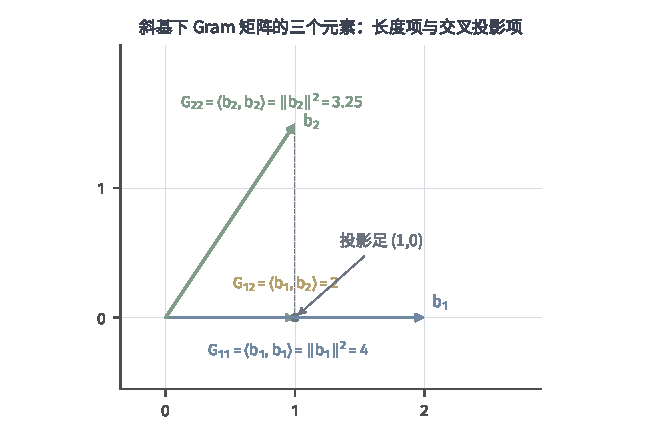
\includegraphics[width=112mm]{figures/00-shared/mathematical-preliminaries-upper/02-linear-spaces/matplotlib/ls-gram-matrix-coefficients/ls-gram-matrix-coefficients.pdf}
  \caption{Gram矩阵把一组基向量的两两内积排成数表。左：平面上两条不垂直的基向量$\bm b_1,\bm b_2$及其夹角；右：$G_{i,j}=\langle\bm b_i,\bm b_j\rangle$构成的$2\times2$Gram矩阵，对角元为各向量长度的平方，非对角元为两向量的内积。基越接近正交，非对角元越接近零；两向量共线时，某个非零组合的平方长度为零，Gram矩阵不再正定。向量与矩阵均为解析教学例。}
  \label{fig:ls-gram-matrix-coefficients}
\end{figure}

\subsubsection{Gram矩阵与半正定矩阵}
\label{sec:ls-gram-semidefinite}

\paragraph{Gram矩阵的半正定性}
Gram矩阵的二次型就是线性组合的长度平方。对任意系数向量$\bm a\in\mathbb R^r$，按双线性展开得
\[
 \bm a^\top\bm G\bm a=\sum_{i,j}a_ia_j\langle\bm b_i,\bm b_j\rangle=\Bigl\lVert\sum_j a_j\bm b_j\Bigr\rVert^2\geq0,
\]
所以Gram矩阵半正定。

Gram矩阵正定，当且仅当只有全零系数使线性组合$\sum_ja_j\bm b_j$为零，即这组向量线性无关（第~\ref{sec:ls-linear-dependence}节）：组合为零时平方长度为零，组合非零时平方长度为正。正定的Gram矩阵可逆：若$\bm G\bm a=\bm0$，则$\bm a^\top\bm G\bm a=0$，从而$\bm a=\bm0$，零空间为零（第~\ref{sec:ls-injective-surjective-invertible}节）。

近共线在Gram矩阵上也有对应的表现。
\begin{example}[近共线两列的Gram矩阵]
\label{ex:ls-nearly-collinear-gram}
给定：贯穿例的两列$\bm c_1,\bm c_2$，取欧氏内积。

计算：由示例~\ref{ex:ls-nearly-collinear-angle}中的三个内积，
\[
\begin{gathered}
\bm G=\bm X_\varepsilon^\top\bm X_\varepsilon=\begin{bmatrix}3&3\\3&3+2\varepsilon^2\end{bmatrix},\\
\bm a^\top\bm G\bm a=3(a_1+a_2)^2+2\varepsilon^2a_2^2 .
\end{gathered}
\]
$\varepsilon\neq0$时，二次型只在$a_1=a_2=0$时为零，所以$\bm G$正定。取$\bm a=(1,-1)^\top$，二次型只有$2\varepsilon^2$；对应的组合$\bm c_1-\bm c_2=-\varepsilon\bm q$确实很短。

结论：$\bm G$正定，与两列线性无关一致；但存在系数使二次型接近零。近共线在Gram矩阵上表现为“正定但几乎退化”。
\end{example}

\paragraph{Gram因子定理}
Gram矩阵总是半正定的。反过来，每个半正定矩阵是否都是某组向量的Gram矩阵？关键是把半正定矩阵的二次型写成欧氏平方和。下面的定理用逐步配方给出这一分解。
\begin{theorem}[半正定矩阵的配方因子]
\label{thm:ls-gram-factor}
设$\bm M\in\mathbb R^{r\times r}$对称半正定，则存在$\bm L\in\mathbb R^{r\times r}$使$\bm M=\bm L^\top\bm L$；若$\bm M$正定，可取$\bm L$可逆。
\end{theorem}
\begin{proof}
对$r$归纳。$r=1$时$\bm M=(m_{1,1})$且$m_{1,1}\geq0$，取$\bm L=(\sqrt{m_{1,1}})$即可。

设$r>1$。若所有对角元都为零，任取$i\neq j$，把$\bm x=\bm e_i+t\bm e_j$代入半正定性：
\[
 0\leq\bm x^\top\bm M\bm x=m_{i,i}+2t\,m_{i,j}+t^2m_{j,j}=2t\,m_{i,j}.
\]
这对正负$t$同时成立，迫使$m_{i,j}=0$，于是$\bm M=\bm0$，取$\bm L=\bm0$。

否则存在正的对角元。取一个置换矩阵$\bm P$把它换到首位（行列同步交换）；$\bm P$的各列是互不相同的标准坐标向量，所以$\bm P^\top\bm P=\bm P\bm P^\top=\bm I$。记
\[
\begin{gathered}
\widetilde{\bm M}=\bm P\bm M\bm P^\top
 =\begin{bmatrix}a&\bm b^\top\\ \bm b&\bm C\end{bmatrix},\\
a>0.
\end{gathered}
\]
$\widetilde{\bm M}$仍对称半正定，因为$\bm x^\top\widetilde{\bm M}\bm x=(\bm P^\top\bm x)^\top\bm M(\bm P^\top\bm x)\geq0$。对第一个变量配方：令$\bm x=(-\bm b^\top\bm u/a,\bm u)$，展开得$\bm x^\top\widetilde{\bm M}\bm x=\bm u^\top(\bm C-\bm b\bm b^\top/a)\bm u\geq0$，故余项$\bm M'=\bm C-\bm b\bm b^\top/a$仍半正定。由归纳假设$\bm M'=\bm L'^\top\bm L'$，取上三角因子
\[
 \widetilde{\bm L}=\begin{bmatrix}\sqrt a&\bm b^\top/\sqrt a\\ \bm0&\bm L'\end{bmatrix},
\]
按分块乘法直接相乘得
\[
 \widetilde{\bm L}^\top\widetilde{\bm L}
 =\begin{bmatrix}a&\bm b^\top\\ \bm b&\bm b\bm b^\top/a+\bm L'^\top\bm L'\end{bmatrix}
 =\widetilde{\bm M}.
\]
换回原矩阵：$\bm M=\bm P^\top\widetilde{\bm M}\bm P=(\widetilde{\bm L}\bm P)^\top(\widetilde{\bm L}\bm P)$，取$\bm L=\widetilde{\bm L}\bm P$即可。

正定时，$\bm M'$也正定（上述$\bm x$在$\bm u\neq\bm0$时非零），由归纳假设$\bm L'$可逆。分块上三角矩阵$\widetilde{\bm L}$的对角块$\sqrt a$与$\bm L'$都可逆，按分块乘法可以直接验证
\[
 \begin{bmatrix}1/\sqrt a&-\bm b^\top\bm L'^{-1}/a\\ \bm0&\bm L'^{-1}\end{bmatrix}
\]
是它的逆。于是$\bm L=\widetilde{\bm L}\bm P$作为可逆矩阵的乘积仍可逆。
\end{proof}
下面对一个二阶正定矩阵按证明的步骤求出因子。
\begin{example}[二阶正定矩阵的配方因子]
\label{ex:ls-gram-factor-two-by-two}
给定：
\[
 \bm M=\begin{bmatrix}4&2\\2&2\end{bmatrix}.
\]

计算：首个对角元$a=4>0$，不需要置换；$\bm b=(2)$，余项$\bm M'=2-2^2/4=1$，取$\bm L'=(1)$。按证明中的分块形式，
\[
 \bm L=\begin{bmatrix}\sqrt a&\bm b^\top/\sqrt a\\ 0&\bm L'\end{bmatrix}=\begin{bmatrix}2&1\\0&1\end{bmatrix}.
\]
直接验证：
\[
 \bm L^\top\bm L=\begin{bmatrix}2&0\\1&1\end{bmatrix}\begin{bmatrix}2&1\\0&1\end{bmatrix}=\begin{bmatrix}4&2\\2&2\end{bmatrix}=\bm M.
\]
相应地，
\[
 \bm x^\top\bm M\bm x=4x_1^2+4x_1x_2+2x_2^2=(2x_1+x_2)^2+x_2^2 .
\]

结论：$\bm M=\bm L^\top\bm L$，且$\bm L$可逆；二次型被写成两个平方之和。
\end{example}
由这个分解，正定矩阵给出的加权长度可写成$\lVert\bm x\rVert_{\bm M}=\lVert\bm L\bm x\rVert_2$：加权内积就是把$\bm x$换成新坐标$\bm L\bm x$后再量欧氏长度。证明中的配方步骤就是第~\ref{sec:ls-cholesky}节Cholesky分解的雏形。

\paragraph{半正定矩阵是Gram矩阵}
因子定理回答了上面的问题：每个半正定矩阵都是某组向量的Gram矩阵。由定理~\ref{thm:ls-gram-factor}，半正定的$\bm M$可写成$\bm M=\bm L^\top\bm L$。记$\bm l_i$为$\bm L$的第$i$列，则$m_{i,j}=\bm l_i^\top\bm l_j=\langle\bm l_i,\bm l_j\rangle$，所以$\bm M$正是$\bm l_1,\ldots,\bm l_r$在欧氏内积下的Gram矩阵。于是“半正定”与“是一组向量的两两内积”说的是同一件事；要判断一个矩阵半正定，可以去找这样一组向量。

\subsubsection{Gram矩阵的逐元素乘法}
\label{sec:ls-schur-product}
利用“半正定矩阵就是Gram矩阵”这一刻画，可以判断两个半正定矩阵的逐元素乘积（第~\ref{sec:ls-hadamard-product}节）是否仍然半正定。

两个半正定矩阵分别是两组向量的Gram矩阵；只要再找到一组向量，使它们的两两内积恰为两个Gram矩阵对应元素之积，就能断定乘积半正定。所得结论称为\term{Schur乘积}定理（Schur product theorem）。
\begin{theorem}[Schur乘积定理]
\label{thm:ls-schur-product}
设$\bm A,\bm B$均为$n$阶对称半正定矩阵，则逐元素乘积$\bm A\odot\bm B$也对称半正定。
\end{theorem}
\begin{proof}
对称性由$(\bm A\odot\bm B)_{k,i}=A_{k,i}B_{k,i}=A_{i,k}B_{i,k}$直接得到。由定理~\ref{thm:ls-gram-factor}，$\bm A=\bm U^\top\bm U$、$\bm B=\bm V^\top\bm V$；记$\bm u_i,\bm v_i$分别为$\bm U,\bm V$的第$i$列，则$A_{i,k}=\langle\bm u_i,\bm u_k\rangle$、$B_{i,k}=\langle\bm v_i,\bm v_k\rangle$。考虑二阶数组$\bm u_1\otimes\bm v_1,\ldots,\bm u_n\otimes\bm v_n$。由Frobenius内积下张量积配对的分离性（第~\ref{sec:ls-tensor-product-properties}节），它们的Gram矩阵为
\[
 \langle\bm u_i\otimes\bm v_i,\bm u_k\otimes\bm v_k\rangle_{\mathrm F}
 =\langle\bm u_i,\bm u_k\rangle\langle\bm v_i,\bm v_k\rangle
 =A_{i,k}B_{i,k}.
\]
所以$\bm A\odot\bm B$是$\bm u_1\otimes\bm v_1,\ldots,\bm u_n\otimes\bm v_n$的Gram矩阵；Gram矩阵恒半正定，故$\bm A\odot\bm B$半正定。
\end{proof}
下面用一个二阶例子核对。
\begin{example}[两个半正定矩阵的逐元素乘积]
\label{ex:ls-schur-product}
给定：
\[
 \bm A=\bm B=\begin{bmatrix}1&1\\1&2\end{bmatrix}.
\]

计算：$\bm A$的二次型为$x_1^2+2x_1x_2+2x_2^2=(x_1+x_2)^2+x_2^2\geq0$，所以$\bm A$半正定。逐元素乘积及其二次型为
\[
\begin{gathered}
\bm A\odot\bm B=\begin{bmatrix}1&1\\1&4\end{bmatrix},\\
x_1^2+2x_1x_2+4x_2^2=(x_1+x_2)^2+3x_2^2\geq0 .
\end{gathered}
\]

结论：$\bm A\odot\bm B$仍半正定，与定理~\ref{thm:ls-schur-product}一致。
\end{example}
核方法中，两个核矩阵的逐元素乘积仍是合法的核矩阵，依据就是这一定理。

\subsubsection{基的Gram矩阵与内积}
\label{sec:ls-gram-coordinates}

选定基以后，一般内积空间上的内积由基的Gram矩阵完全确定。

设$\mathcal B=(\bm b_1,\ldots,\bm b_d)$是$V$的基，$\bm G$是它的Gram矩阵。

对$\bm v=\sum_ix_i\bm b_i$、$\bm w=\sum_jy_j\bm b_j$，按双线性展开得
\[
 \langle\bm v,\bm w\rangle=\sum_{i,j}x_iy_j\langle\bm b_i,\bm b_j\rangle=[\bm v]_{\mathcal B}^\top\,\bm G\,[\bm w]_{\mathcal B}.
\]

基线性无关，所以$\bm G$对称正定。

因此在坐标下，任一内积都是以$\bm G$为权重的加权内积。特别地，$\mathbb R^d$上的任一内积在标准基下都是$\bm x^\top\bm G\bm y$，其中$g_{i,j}=\langle\bm e_i,\bm e_j\rangle$。

反过来，每个对称正定矩阵都给出一个加权内积。所以$\mathbb R^d$上的内积与$d$阶对称正定矩阵一一对应，欧氏内积对应$\bm I$。下面用示例~\ref{ex:ls-two-point-inner-product}的内积核对坐标公式。
\begin{example}[两点内积的坐标计算]
\label{ex:ls-two-point-inner-product-coordinates}
给定：示例~\ref{ex:ls-two-point-inner-product}中$P_1$上的内积$\langle f,g\rangle=f(0)g(0)+f(1)g(1)$，基$(1,t)$，以及$f=1+t$、$g=1-2t$。

计算：由$\langle1,1\rangle=1\cdot1+1\cdot1=2$、$\langle1,t\rangle=1\cdot0+1\cdot1=1$、$\langle t,t\rangle=0\cdot0+1\cdot1=1$，基的Gram矩阵为
\[
 \bm G=\begin{bmatrix}2&1\\1&1\end{bmatrix}.
\]
按定义，$f$在$t=0,1$处取值$1,2$，$g$取值$1,-1$，所以$\langle f,g\rangle=1\cdot1+2\cdot(-1)=-1$。按坐标，$[f]=(1,1)^\top$、$[g]=(1,-2)^\top$，
\[
 (1,1)\,\bm G\begin{bmatrix}1\\-2\end{bmatrix}=(3,2)\begin{bmatrix}1\\-2\end{bmatrix}=-1 .
\]

结论：两种算法给出同一个内积值$-1$。
\end{example}
若基两两正交且长度为$1$，则$\bm G=\bm I$，内积在坐标下就是欧氏内积；这样的基在第~\ref{sec:ls-orthonormal-bases}节讨论。

\paragraph{合同变换} 
换基时，Gram矩阵按另一种规则变化。若旧坐标与新坐标满足$\bm x=\bm C\widetilde{\bm x}$，内积中的两个坐标都要改变，因此Gram矩阵变为
\[
 \widetilde{\bm G}=\bm C^\top\bm G\bm C.
\]
这称为合同变换，它保持同一个内积与二次型。相似变换记录的则是同一个算子的换基，两者用途不同。

\subsubsection{复空间中的Gram矩阵}
\label{sec:ls-complex-gram}

前面的Gram矩阵都在实内积空间中讨论。按第~\ref{sec:ls-inner-product-axioms}节的约定，复内积对第一个变量共轭线性、对第二个变量线性，并满足$\langle\bm x,\bm y\rangle=\overline{\langle\bm y,\bm x\rangle}$。对复内积空间中的向量$\bm b_1,\ldots,\bm b_k$，Gram矩阵仍定义为$G_{i,j}=\langle\bm b_i,\bm b_j\rangle$。下面说明哪些结论照样成立，哪些需要修改。

\paragraph{自共轭代替对称}
实空间中，内积的对称性使Gram矩阵对称。复空间中，交换两个变量要取共轭：
\[
 G_{j,i}=\langle\bm b_j,\bm b_i\rangle=\overline{\langle\bm b_i,\bm b_j\rangle}=\overline{G_{i,j}},
\]
即$\bm G^*=\bm G$，其中$\bm G^*$是共轭转置。满足$\bm G^*=\bm G$的矩阵称为\term{自共轭矩阵}（Hermitian matrix），第~\ref{sec:ls-adjoints}节从伴随的角度称它为自伴矩阵。它的对角元$G_{i,i}=\lVert\bm b_i\rVert^2$是实数，非对角元一般是复数；$\bm G$一般不对称，$\bm G^\top=\overline{\bm G}$。实Gram矩阵是自共轭矩阵的特例，因为实矩阵的共轭转置就是转置。

\paragraph{半正定性照样成立}
对复系数向量$\bm c\in\mathbb C^k$，由内积对第一个变量共轭线性、对第二个变量线性，
\[
 \bm c^*\bm G\bm c=\sum_{i,j}\overline{c_i}\,c_j\langle\bm b_i,\bm b_j\rangle
 =\Bigl\langle\sum_ic_i\bm b_i,\sum_jc_j\bm b_j\Bigr\rangle
 =\Bigl\lVert\sum_jc_j\bm b_j\Bigr\rVert^2\geq0 .
\]
这与实情形的等式完全相同，只是左端的转置换成了共轭转置。自共轭矩阵的$\bm c^*\bm G\bm c$总是实数，所以“非负”有意义；称满足$\bm c^*\bm G\bm c\geq0$的自共轭矩阵为半正定。于是复Gram矩阵总是半正定的。

\paragraph{正定与线性无关的关系照样成立}
由同一等式，$\bm c^*\bm G\bm c=0$当且仅当$\sum_jc_j\bm b_j=\bm0$。所以$\bm G$正定，即$\bm c\neq\bm0$时$\bm c^*\bm G\bm c>0$，当且仅当$\bm b_1,\ldots,\bm b_k$在复数域上线性无关。这里的线性无关允许复系数：在实数域上无关的一组向量，在复数域上可能相关。例如在$\mathbb C$中，$1$与$\mathrm i$在实系数下无关，但$\mathrm i\cdot1-\mathrm i=0$，在复系数下相关；对应的Gram矩阵$\begin{bmatrix}1&\mathrm i\\-\mathrm i&1\end{bmatrix}$的行列式为$1-1=0$，确实不是正定的。

逐步配方的证明也保留。分块
\[
 \bm G=\begin{bmatrix}a&\bm b^*\\\bm b&\bm C\end{bmatrix}
\]
且$a>0$时，分离出的平方项为$a|z+\bm b^*\bm y/a|^2$，剩余矩阵是$\bm C-\bm b\bm b^*/a$；若对角元全为零，取只有两个分量非零且相位可调的向量，半正定性迫使所有非对角元也为零。递推便得到$\bm G=\bm L^*\bm L$：每个半正定的自共轭矩阵都是某组向量的Gram矩阵，不需要借用后面的谱定理。

\paragraph{坐标下的内积与换基}
在一组基下，复内积写成$\langle\bm x,\bm y\rangle=\bm x^*\bm G\bm y$，其中$\bm x,\bm y$表示坐标，$\bm G$是基的Gram矩阵，它是正定的自共轭矩阵。换基$\bm x=\bm C\widetilde{\bm x}$时，两个坐标都要改变，Gram矩阵变为$\bm C^*\bm G\bm C$，合同变换中的转置相应换成共轭转置。
\begin{example}[复空间中的Gram矩阵]
\label{ex:ls-complex-gram}
给定：$\mathbb C^2$取标准内积$\langle\bm x,\bm y\rangle=\bm x^*\bm y$，向量$\bm b_1=(1,\mathrm i)^\top$、$\bm b_2=(1,1)^\top$。

计算：$\langle\bm b_1,\bm b_1\rangle=1+|\mathrm i|^2=2$，$\langle\bm b_2,\bm b_2\rangle=2$，$\langle\bm b_1,\bm b_2\rangle=\overline1\cdot1+\overline{\mathrm i}\cdot1=1-\mathrm i$，$\langle\bm b_2,\bm b_1\rangle=1+\mathrm i$，所以
\[
 \bm G=\begin{bmatrix}2&1-\mathrm i\\1+\mathrm i&2\end{bmatrix}.
\]
它不对称，但$\bm G^*=\bm G$。对角元为正，$\det\bm G=4-|1-\mathrm i|^2=2>0$，所以$\bm G$正定，与$\bm b_1,\bm b_2$线性无关一致。

结论：复Gram矩阵是自共轭矩阵而不一定对称；半正定性以及正定与线性无关的对应，都与实情形相同。
\end{example}

\section{正交与投影}
\label{sec:ls-orthogonality-and-projection}

内积给出了两个向量之间的正交关系。本节把它推广到向量与子空间之间，把向量分解为子空间中的分量与和子空间正交的剩余部分。接着引入标准正交基，并用Gram--Schmidt正交化构造它；最后用标准正交基写出正交投影，证明它给出唯一的最近点。

\subsection{正交补与正交分解}
\label{sec:ls-orthogonality}

Gram矩阵记录的是一组向量两两之间是否正交。本小节考虑一个向量与整个子空间的正交，由此得到一个由内积唯一确定的补空间，并用它证明四个基本子空间之间的垂直关系。

\paragraph{正交补}
第~\ref{sec:ls-direct-sum}节说明，一个子空间的补空间一般不唯一。有了内积，可以挑出一个由垂直关系确定的补空间。设$U$是有限维内积空间$V$的子空间，与$U$中每个向量都正交的向量组成集合
\[
 U^\perp=\{\bm r\in V:\langle\bm u,\bm r\rangle=0,\ \forall\bm u\in U\},
\]
称为$U$的\term{正交补}（orthogonal complement）。由内积的双线性，$U^\perp$对线性组合封闭，是子空间。要检查$\bm r\in U^\perp$，只需检查它与$U$的一组基逐个正交，因为与基向量都正交的向量，也与基向量的每个组合正交。

\paragraph{正交直和}
下面证明正交补确实是一个补空间，而且分解可以由Gram矩阵算出。
\begin{lemma}[正交直和]
\label{lem:ls-orthogonal-decomposition}
设$U$是有限维内积空间$V$的子空间，则每个$\bm x\in V$唯一分解为$\bm x=\bm u+\bm r$，其中$\bm u\in U$、$\bm r\in U^\perp$；即$V=U\oplus U^\perp$。
\end{lemma}
\begin{proof}
取$U$的一组基$\bm b_1,\ldots,\bm b_r$。它线性无关，所以Gram矩阵$\bm G$正定，从而可逆。对任意$\bm x$，令$\bm u=\sum_j a_j\bm b_j$，并要求$\bm r=\bm x-\bm u$与每个$\bm b_i$正交，得到系数方程
\[
 \begin{gathered}
\sum_j g_{i,j}a_j=\langle\bm b_i,\bm x\rangle,\\
i=1,\ldots,r,
 \end{gathered}
\]
即$\bm G\bm a=(\langle\bm b_i,\bm x\rangle)_i$。$\bm G$可逆，所以系数唯一解出；残差$\bm r$与全部基向量正交，因而落在$U^\perp$。

若$\bm x=\bm u+\bm r=\bm u'+\bm r'$是两种分解，则$\bm u-\bm u'=\bm r'-\bm r$同时属于$U$与$U^\perp$。它与自身正交，长度为零，故两种分解相同。
\end{proof}
所以正交补是$U$的一个补空间，并且由内积唯一确定；$V=U\oplus U^\perp$称为正交直和。由维数公式，$\dim U^\perp=\dim V-\dim U$。下面在$\mathbb R^3$中做一次分解。
\begin{example}[向一条直线的正交分解]
\label{ex:ls-orthogonal-decomposition-line}
给定：$\mathbb R^3$取欧氏内积，$U=\operatorname{span}\{\bm c_1\}$，$\bm c_1=(1,1,1)^\top$，$\bm y=(1,1.1,0.9)^\top$。

计算：$U^\perp$由与$\bm c_1$正交的向量组成，即坐标和为零的平面。$U$只有一个基向量，Gram方程只有一个未知数：$\langle\bm c_1,\bm c_1\rangle a=\langle\bm c_1,\bm y\rangle$，即$3a=3$，所以$a=1$。于是
\[
 \begin{gathered}
 \bm u=\bm c_1=(1,1,1)^\top,
 \\
 \bm r=\bm y-\bm u=(0,0.1,-0.1)^\top,
 \end{gathered}
\]
$\bm r$的坐标和为零，确实属于$U^\perp$。

结论：$\bm y=\bm u+\bm r$就是$\bm y$在正交直和$\mathbb R^3=U\oplus U^\perp$中的分解。
\end{example}
这里只得到了正交分量的存在与唯一。它为什么是$U$中离$\bm y$最近的点，将在第~\ref{sec:ls-orthogonal-projection}节用标准正交基证明。

取两次正交补会回到原来的子空间：$(U^\perp)^\perp=U$。一方面，$U$中每个向量与$U^\perp$中每个向量正交，所以$U\subseteq(U^\perp)^\perp$。另一方面，对$U^\perp$用上面的维数关系，$\dim(U^\perp)^\perp=\dim V-\dim U^\perp=\dim U$。二者包含且同维，由第~\ref{sec:ls-dimension}节，两者相等。

\paragraph{四个基本子空间的正交关系}
示例~\ref{ex:ls-rank-one-four-subspaces}显示，行空间的方向与零空间垂直，列空间的方向与左零空间垂直。现在在$\mathbb R^d$与$\mathbb R^m$上取欧氏内积，证明这对任何矩阵都成立。
\begin{theorem}[四个基本子空间的正交关系]
\label{thm:ls-four-subspaces-orthogonality}
设$\bm A\in\mathbb R^{m\times d}$，$\mathbb R^d$与$\mathbb R^m$取欧氏内积。则
\begin{equation}
\begin{gathered}
\operatorname{null}(\bm A)=\operatorname{range}(\bm A^\top)^\perp,\\
\operatorname{null}(\bm A^\top)=\operatorname{range}(\bm A)^\perp,
\end{gathered}
\label{eq:ls-four-subspaces-orthogonality}
\end{equation}
因而有正交直和
\begin{equation}
\begin{gathered}
\mathbb R^d=\operatorname{range}(\bm A^\top)\oplus\operatorname{null}(\bm A),\\
\mathbb R^m=\operatorname{range}(\bm A)\oplus\operatorname{null}(\bm A^\top).
\end{gathered}
\label{eq:ls-four-subspaces-decomposition}
\end{equation}
\end{theorem}
\begin{proof}
由转置的乘积规则（第~\ref{sec:ls-reshaping}节），对任意$\bm x\in\mathbb R^d$、$\bm y\in\mathbb R^m$，
\[
 \langle\bm A\bm x,\bm y\rangle=(\bm A\bm x)^\top\bm y=\bm x^\top(\bm A^\top\bm y)=\langle\bm x,\bm A^\top\bm y\rangle.
\]
$\bm y\in\operatorname{range}(\bm A)^\perp$意味着左端对一切$\bm x$为零，即右端对一切$\bm x$为零；取$\bm x=\bm A^\top\bm y$可见，这当且仅当$\bm A^\top\bm y=\bm0$。所以$\operatorname{range}(\bm A)^\perp=\operatorname{null}(\bm A^\top)$。把$\bm A$换成$\bm A^\top$，得$\operatorname{range}(\bm A^\top)^\perp=\operatorname{null}(\bm A)$。正交直和由引理~\ref{lem:ls-orthogonal-decomposition}得到。
\end{proof}
两边再取正交补，并用$(U^\perp)^\perp=U$，还得到$\operatorname{null}(\bm A)^\perp=\operatorname{range}(\bm A^\top)$、$\operatorname{null}(\bm A^\top)^\perp=\operatorname{range}(\bm A)$。于是输入空间分成两块互相垂直的部分：零空间是被$\bm A$消去的方向，行空间是真正影响输出的方向。输出空间也分成两块：列空间是能够到达的输出，左零空间中的方向则无论输入取什么都无法到达。

这一定理与第~\ref{sec:ls-kernel-image}节的维数关系相互印证。由正交直和与秩零度定理，分别得到
\[
 \begin{gathered}
d=\dim\operatorname{range}(\bm A^\top)+\dim\operatorname{null}(\bm A),\\
d=\operatorname{rank}\bm A+\dim\operatorname{null}(\bm A).
 \end{gathered}
\]
两式比较，又一次得到行秩等于列秩。示例~\ref{ex:ls-rank-one-four-subspaces}中逐项相乘再相加得零的观察，现在由定理得到了解释。

输出端的分解还给出方程$\bm A\bm x=\bm b$有解的一个判据：$\bm b\in\operatorname{range}(\bm A)$，当且仅当$\bm b$与左零空间中每个向量正交。第~\ref{chap:linear-equations-and-optimization}章判断方程是否有解时会用到这一点。

\subsection{标准正交基}
\label{sec:ls-orthonormal-bases}

前面的计算都要用到Gram矩阵：正交分解要解Gram方程$\bm G\bm a=(\langle\bm b_i,\bm x\rangle)_i$，坐标下的内积要乘Gram矩阵。示例~\ref{ex:ls-coordinate-instability}还显示，接近共线的基会把小的对象记成很大的系数。这些麻烦都来自Gram矩阵的非对角元，即基向量之间的相互干扰。本小节研究Gram矩阵为单位矩阵的基：先证明它确实是一组基，再给出它下的坐标、对应的正交矩阵，以及这类基之间的换基。

\paragraph{标准正交基的定义}
一组向量$\bm q_1,\ldots,\bm q_r$若满足
\[
 \langle\bm q_i,\bm q_j\rangle=\delta_{i,j}=\begin{cases}1,&i=j,\\0,&i\neq j,\end{cases}
\]
即两两正交且长度都为$1$，就称为标准正交组；它的Gram矩阵是$\bm I_r$。张成子空间$U$的标准正交组称为$U$的\term{标准正交基}（orthonormal basis）；$U=V$时就是$V$的标准正交基。

在$\mathbb R^m$中取欧氏内积，把$r$个向量排成$\bm Q\in\mathbb R^{m\times r}$的各列，它们的Gram矩阵是$\bm Q^\top\bm Q$，所以标准正交的条件就是$\bm Q^\top\bm Q=\bm I_r$。$r=m$时，$\bm Q$是下面定义的正交矩阵。$r<m$时，$\bm Q^\top\bm Q=\bm I_r$仍成立，但$\bm Q\bm Q^\top$的秩只有$r$，不等于$\bm I_m$，$\bm Q$只有左逆$\bm Q^\top$。

\paragraph{标准正交组构成基}
标准正交组总是线性无关。设$\sum_jc_j\bm q_j=\bm0$，两边与$\bm q_i$作内积。左边每一项$c_j\langle\bm q_j,\bm q_i\rangle$只在$j=i$时不为零，于是$c_i=0$；$i$任意，所以全部系数为零。同样的论证说明两两正交的非零向量组线性无关，只是最后一步改为由$c_i\langle\bm q_i,\bm q_i\rangle=0$与$\langle\bm q_i,\bm q_i\rangle>0$得$c_i=0$。

因此标准正交组是它所张成子空间的一组基。在$d$维内积空间中，$d$个两两正交的单位向量的个数等于维数，自动构成整个空间的标准正交基，不必另行验证张成。例如，$\mathbb R^d$的标准基在欧氏内积下是标准正交基；$\bm q_1=(1,1)^\top/\sqrt2$、$\bm q_2=(1,-1)^\top/\sqrt2$是$\mathbb R^2$的另一组标准正交基。

\paragraph{标准正交基下的坐标}
在标准正交基下，求坐标不必解方程。若$\bm v=\sum_jc_j\bm q_j$，两边与$\bm q_i$作内积，右边只剩$c_i$一项，所以
\begin{equation}
 \bm v=\sum_{j=1}^d\langle\bm v,\bm q_j\rangle\,\bm q_j.
 \label{eq:ls-orthonormal-expansion}
\end{equation}
每个系数只与自己的方向有关，增加或删去其他方向都不改变它。坐标下的内积变成欧氏内积：$\langle\bm v,\bm w\rangle=\sum_jc_jd_j$，其中$c_j,d_j$分别是$\bm v,\bm w$的坐标。特别地，
\begin{equation}
 \lVert\bm v\rVert^2=\sum_{j=1}^d\langle\bm v,\bm q_j\rangle^2,
 \label{eq:ls-parseval}
\end{equation}
即长度的平方等于各坐标的平方和。这称为Parseval恒等式，是勾股定理在$d$个互相垂直方向上的推广。下面用平面上的一组标准正交基验证这两点。
\begin{example}[标准正交基下的坐标与Parseval恒等式]
\label{ex:ls-orthonormal-coordinates}
给定：$\mathbb R^2$的标准正交基$\bm q_1=(1,1)^\top/\sqrt2$、$\bm q_2=(1,-1)^\top/\sqrt2$，向量$\bm v=(3,1)^\top$。

计算：由式~\eqref{eq:ls-orthonormal-expansion}，坐标为$\langle\bm v,\bm q_1\rangle=4/\sqrt2=2\sqrt2$与$\langle\bm v,\bm q_2\rangle=2/\sqrt2=\sqrt2$，不必解方程。坐标的平方和为$8+2=10$，而$\lVert\bm v\rVert^2=3^2+1^2=10$。

结论：坐标由内积直接读出，平方和等于长度的平方。
\end{example}
由Parseval恒等式，坐标的大小如实反映对象的大小，近共线基下“小对象、大系数”的现象不会发生。

\paragraph{正交矩阵}
\phantomsection
\label{sec:ls-orthogonal-matrices}
在$\mathbb R^n$中，以一组标准正交基为列的方阵有专门的名称。若$n$阶方阵$\bm Q$的各列都是单位向量，并且两两正交，就称它为\term{正交矩阵}（orthogonal matrix）。单位矩阵和置换矩阵都是正交矩阵，因为它们的列是互不相同的标准坐标向量。

下面检验平面旋转矩阵满足这一定义，并说明只有各列两两正交还不够。
\begin{example}[平面旋转是正交矩阵]
\label{ex:ls-rotation-orthogonal}
给定：任一实数$\phi$对应的平面旋转矩阵
\[
 \bm R_\phi=\begin{bmatrix}\cos\phi&-\sin\phi\\\sin\phi&\cos\phi\end{bmatrix},
\]
以及对角矩阵$\operatorname{diag}(2,1)$。
验证：$\bm R_\phi$两列的长度与内积分别为
\[
 \begin{gathered}
\sqrt{\cos^2\phi+\sin^2\phi}=1,\\
\cos\phi\cdot(-\sin\phi)+\sin\phi\cdot\cos\phi=0.
 \end{gathered}
\]
$\operatorname{diag}(2,1)$的两列$(2,0)^\top$与$(0,1)^\top$内积为零，但第一列长度为$2$。
结论：$\bm R_\phi$是正交矩阵；$\operatorname{diag}(2,1)$的各列两两正交，却不是正交矩阵，因为正交矩阵还要求每列长度为$1$。
\end{example}
逐列检验长度和内积比较繁琐。下面先把定义改写成一个矩阵等式，再由它推出正交矩阵的各项性质。

\paragraph{正交矩阵的转置条件}
$n$阶方阵$\bm Q$是正交矩阵，当且仅当
\[
 \bm Q^\top\bm Q=\bm I_n.
\]
这是因为$(\bm Q^\top\bm Q)_{i,j}$是$\bm Q$的第$i$列与第$j$列的内积。“各列都是单位向量”对应对角元等于$1$，“各列两两正交”对应非对角元等于$0$，两者合起来正是这个矩阵等式。下面用这个条件重新检验示例~\ref{ex:ls-rotation-orthogonal}中的两个矩阵。
\begin{example}[用转置条件检验正交矩阵]
\label{ex:ls-orthogonality-by-transpose}
给定：旋转矩阵$\bm R_\phi$与对角矩阵$\operatorname{diag}(2,1)$。
计算：
\[
 \begin{aligned}
 \bm R_\phi^\top\bm R_\phi
 &=\begin{bmatrix}\cos\phi&\sin\phi\\-\sin\phi&\cos\phi\end{bmatrix}
   \begin{bmatrix}\cos\phi&-\sin\phi\\\sin\phi&\cos\phi\end{bmatrix}\\
 &=\begin{bmatrix}\cos^2\phi+\sin^2\phi&0\\0&\sin^2\phi+\cos^2\phi\end{bmatrix}
 =\bm I_2,\\
 \operatorname{diag}(2,1)^\top\operatorname{diag}(2,1)&=\operatorname{diag}(4,1)\neq\bm I_2.
 \end{aligned}
\]
结论：$\bm R_\phi$满足转置条件，是正交矩阵；$\operatorname{diag}(2,1)$的乘积在$(1,1)$位置为$4\neq1$，对应第一列长度不为$1$。
\end{example}

\paragraph{正交矩阵保持内积}
由内积中的转置与转置条件，
\[
 \langle\bm Q\bm x,\bm Q\bm y\rangle=\langle\bm x,\bm Q^\top\bm Q\bm y\rangle=\langle\bm x,\bm y\rangle\qquad(\bm Q\text{为正交矩阵}).
\]
特别地，正交矩阵把两两正交的向量仍送到两两正交的向量。

\paragraph{正交矩阵的乘法}
若$\bm Q_1,\bm Q_2$是$n$阶正交矩阵，则
\[
 (\bm Q_1\bm Q_2)^\top(\bm Q_1\bm Q_2)=\bm Q_2^\top\bm Q_1^\top\bm Q_1\bm Q_2=\bm Q_2^\top\bm Q_2=\bm I_n,
\]
由转置条件，$\bm Q_1\bm Q_2$仍是正交矩阵。下面的例子显示，两个平面旋转的乘积不仅是正交矩阵，而且仍是旋转。
\begin{example}[两个平面旋转的乘积]
\label{ex:ls-rotation-composition}
给定：旋转矩阵$\bm R_\phi$与$\bm R_\psi$。
计算：直接相乘，再用和角公式$\cos(\phi+\psi)=\cos\phi\cos\psi-\sin\phi\sin\psi$与$\sin(\phi+\psi)=\sin\phi\cos\psi+\cos\phi\sin\psi$，得
\[
 \begin{aligned}
 \bm R_\phi\bm R_\psi
 &=\begin{bmatrix}\cos\phi\cos\psi-\sin\phi\sin\psi&-\cos\phi\sin\psi-\sin\phi\cos\psi\\\sin\phi\cos\psi+\cos\phi\sin\psi&-\sin\phi\sin\psi+\cos\phi\cos\psi\end{bmatrix}\\
 &=\bm R_{\phi+\psi}.
 \end{aligned}
\]
结论：先转$\psi$角、再转$\phi$角，等于一次转$\phi+\psi$角；乘积是正交矩阵，与上面的一般结论一致。
\end{example}

\paragraph{正交矩阵的逆}
正交矩阵求逆只需转置：
\[
\begin{gathered}
\bm Q^{-1}=\bm Q^\top,\\
\bm Q\bm Q^\top=\bm I_n\qquad(\bm Q\text{为正交矩阵}).
\end{gathered}
\]
转置条件$\bm Q^\top\bm Q=\bm I_n$只说明$\bm Q^\top$是$\bm Q$的左逆。方阵只要有一侧的逆就可逆，而且这个单侧逆就是逆矩阵；这一点的证明要用到行列式，放在第~\ref{sec:ls-square-one-sided-inverse}节。由此$\bm Q^{-1}=\bm Q^\top$，另一侧的乘积$\bm Q\bm Q^\top$也等于$\bm I_n$。

$\bm Q\bm Q^\top$的$(i,j)$元是$\bm Q$的第$i$行与第$j$行的内积，所以正交矩阵的各行同样两两正交且长度为$1$。又因$(\bm Q^\top)^\top\bm Q^\top=\bm Q\bm Q^\top=\bm I_n$，由转置条件，$\bm Q^{-1}=\bm Q^\top$也是正交矩阵。

\paragraph{正交矩阵的行列式}
正交矩阵的行列式只能取两个值：
\[
 \det\bm Q=\pm1\qquad(\bm Q\text{为正交矩阵}).
\]
由$\det(\bm Q^\top)\det\bm Q=\det(\bm Q^\top\bm Q)=\det\bm I_n=1$及$\det(\bm Q^\top)=\det\bm Q$，得$(\det\bm Q)^2=1$。旋转$\bm R_\phi$的行列式为$\cos^2\phi+\sin^2\phi=1$；交换两个坐标的置换矩阵行列式为$-1$，它翻转了定向。

\paragraph{标准正交基之间的换基}
正交矩阵也出现在标准正交基之间的换基中。设$\mathcal B=(\bm b_1,\ldots,\bm b_d)$与$\mathcal C$都是$V$的标准正交基，换基矩阵$\bm S=\bm S_{\mathcal C\leftarrow\mathcal B}$的第$j$列是$\bm b_j$的$\mathcal C$坐标。在标准正交基$\mathcal C$下，内积就是坐标的欧氏内积，所以$\bm S$的第$i$、$j$两列的欧氏内积等于$\langle\bm b_i,\bm b_j\rangle=\delta_{i,j}$，即$\bm S^\top\bm S=\bm I$。因此两组标准正交基之间的换基矩阵是正交矩阵。

于是反向换基只需转置，$\bm S^{-1}=\bm S^\top$，不会出现示例~\ref{ex:ls-nearly-collinear-change-of-basis}中除以小数$\varepsilon$的放大。例如从上面的$(\bm q_1,\bm q_2)$换到标准基，换基矩阵的两列就是$\bm q_1,\bm q_2$本身。对线性算子，若只在标准正交基之间换基，相似关系$\bm B=\bm P^{-1}\bm A\bm P$变成$\bm B=\bm P^\top\bm A\bm P$。第~\ref{chap:linear-analysis}章的谱定理就是在这种受限的换基下化简对称矩阵。

\paragraph{正交不变性}
正交矩阵保持欧氏长度，因此也不改变与欧氏长度相关的矩阵范数。设$\bm Q$为正交矩阵，则
\[
 \begin{gathered}
 \lVert\bm Q\bm x\rVert_2=\lVert\bm x\rVert_2,\\
 \lVert\bm Q\rVert_2=1,
 \end{gathered}
\]
\[
 \begin{gathered}
 \lVert\bm Q\bm A\rVert_{\mathrm F}=\lVert\bm A\rVert_{\mathrm F},\\
 \lVert\bm Q\bm A\rVert_2=\lVert\bm A\rVert_2.
 \end{gathered}
\]
由$\lVert\bm Q\bm x\rVert_2^2=\bm x^\top\bm Q^\top\bm Q\bm x=\lVert\bm x\rVert_2^2$，正交矩阵保持欧氏长度，所以每个比值$\lVert\bm Q\bm x\rVert_2/\lVert\bm x\rVert_2$都等于$1$，$\lVert\bm Q\rVert_2=1$。对矩阵$\bm A$，左乘$\bm Q$不改变各列的长度，$\lVert\bm Q\bm A_{:,j}\rVert_2=\lVert\bm A_{:,j}\rVert_2$，对$j$求平方和即得$\lVert\bm Q\bm A\rVert_{\mathrm F}=\lVert\bm A\rVert_{\mathrm F}$。左乘$\bm Q$也不改变每个输出的长度，$\lVert\bm Q\bm A\bm x\rVert_2=\lVert\bm A\bm x\rVert_2$，取上确界即得$\lVert\bm Q\bm A\rVert_2=\lVert\bm A\rVert_2$。

\subsection{Gram--Schmidt正交化}
\label{sec:ls-orthonormal-basis-construction}

本小节说明，任意一组线性无关的向量都可以改造成标准正交组。思路来自正交分解：依次处理各向量，从每个向量中扣除它在已经得到的方向上的分量，剩下的部分与这些方向都垂直，再把它缩放到单位长度。下面先给出这一过程并证明它总能完成，再把它在$\mathbb R^m$中写成矩阵分解，最后处理各列线性相关的情形。

\subsubsection{Gram--Schmidt正交化}

这一过程称为\term{Gram--Schmidt正交化}（Gram--Schmidt orthogonalization），也称施密特正交化。设$\bm v_1,\ldots,\bm v_k$线性无关。令$\bm u_1=\bm v_1$、$\bm q_1=\bm u_1/\lVert\bm u_1\rVert$；对$j=2,\ldots,k$依次令
\begin{equation}
\begin{gathered}
\bm u_j=\bm v_j-\sum_{i=1}^{j-1}\langle\bm v_j,\bm q_i\rangle\bm q_i,\\
\bm q_j=\frac{\bm u_j}{\lVert\bm u_j\rVert}.
\end{gathered}
\label{eq:ls-gram-schmidt}
\end{equation}
扣除的部分在$\operatorname{span}\{\bm q_1,\ldots,\bm q_{j-1}\}$中，剩下的$\bm u_j$与这些方向都正交，所以$\bm u_j$正是正交分解中的剩余分量。下面的定理验证这一点，并说明过程不会中断。
\begin{theorem}[Gram--Schmidt正交化]
\label{thm:ls-gram-schmidt}
上述过程中每个$\bm u_j\neq\bm0$，得到的$\bm q_1,\ldots,\bm q_k$两两正交、长度为$1$，并且对每个$j$都有$\operatorname{span}\{\bm q_1,\ldots,\bm q_j\}=\operatorname{span}\{\bm v_1,\ldots,\bm v_j\}$。
\end{theorem}
\begin{proof}
对$j$归纳。$j=1$时$\bm u_1=\bm v_1\neq\bm0$，结论成立。设结论对$j-1$成立。对$i<j$，由$\bm q_1,\ldots,\bm q_{j-1}$两两正交且长度为$1$，
\[
 \langle\bm u_j,\bm q_i\rangle=\langle\bm v_j,\bm q_i\rangle-\langle\bm v_j,\bm q_i\rangle\langle\bm q_i,\bm q_i\rangle=0,
\]
所以$\bm u_j$与前面的方向都正交。若$\bm u_j=\bm0$，则$\bm v_j$落在前$j-1$个新方向的张成空间中。由归纳假设，这也是前$j-1$个原向量的张成空间，与线性无关矛盾；故$\bm u_j\neq\bm0$，$\bm q_j$有定义且长度为$1$。最后，$\bm q_j$是$\bm v_j$与$\bm q_1,\ldots,\bm q_{j-1}$的组合，因而属于$\operatorname{span}\{\bm v_1,\ldots,\bm v_j\}$；反过来，由式~\eqref{eq:ls-gram-schmidt}，$\bm v_j=\lVert\bm u_j\rVert\bm q_j+\sum_{i<j}\langle\bm v_j,\bm q_i\rangle\bm q_i$属于$\operatorname{span}\{\bm q_1,\ldots,\bm q_j\}$。两个张成空间互相包含，因而相等。
\end{proof}
对有限维内积空间的任意一组基作Gram--Schmidt正交化，就得到一组标准正交基，所以\emph{每个有限维内积空间都有标准正交基}。若已有几个两两正交的单位向量，可以先把它们扩充成一组基，再从它们之后开始正交化。前面的向量在过程中保持不变，所以任何标准正交组都能扩充成标准正交基。

张成空间逐段相等也有用处：前$j$个新方向与前$j$个旧方向张成同一个子空间，正交化只是在每一段内部换了一组更好用的基。

\paragraph{算例}
标准正交基依赖内积；换一个内积，同一组基正交化的结果也不同。下面在示例~\ref{ex:ls-two-point-inner-product}的内积下对基$(1,t)$作正交化。在这个内积下$\langle1,t\rangle=1\neq0$，两个基向量并不正交。
\begin{example}[两点内积下的Gram--Schmidt正交化]
\label{ex:ls-gram-schmidt-two-point}
给定：$P_1$上的内积$\langle f,g\rangle=f(0)g(0)+f(1)g(1)$，基$(1,t)$。

计算：第一步，归一化第一个基向量。$\lVert1\rVert^2=1^2+1^2=2$，所以
\[
 q_1=\frac1{\sqrt2}.
\]

第二步，从第二个基向量中扣除它在$q_1$上的分量。$\langle t,q_1\rangle=\bigl(0\cdot1+1\cdot1\bigr)/\sqrt2=1/\sqrt2$，所以
\[
 u_2=t-\langle t,q_1\rangle q_1=t-\frac1{\sqrt2}\cdot\frac1{\sqrt2}=t-\frac12.
\]

第三步，归一化。$u_2$在$t=0,1$处的取值为$-\tfrac12,\tfrac12$，所以$\lVert u_2\rVert^2=\tfrac14+\tfrac14=\tfrac12$，
\[
 q_2=\frac{u_2}{\lVert u_2\rVert}=\sqrt2\Bigl(t-\frac12\Bigr).
\]

第四步，核对。$q_1$在$t=0,1$处取值都是$\tfrac1{\sqrt2}$，$q_2$取值为$-\tfrac{\sqrt2}2,\tfrac{\sqrt2}2$，所以$\langle q_1,q_2\rangle=\tfrac1{\sqrt2}\cdot\bigl(-\tfrac{\sqrt2}2\bigr)+\tfrac1{\sqrt2}\cdot\tfrac{\sqrt2}2=0$，$\lVert q_2\rVert^2=\tfrac12+\tfrac12=1$。

第五步，用新基读坐标。$f=1+t$在$t=0,1$处取值为$1,2$，所以$\langle f,q_1\rangle=(1+2)/\sqrt2=3/\sqrt2$，$\langle f,q_2\rangle=1\cdot\bigl(-\tfrac{\sqrt2}2\bigr)+2\cdot\tfrac{\sqrt2}2=\tfrac{\sqrt2}2$。还原得$\tfrac3{\sqrt2}\cdot\tfrac1{\sqrt2}+\tfrac{\sqrt2}2\cdot\sqrt2(t-\tfrac12)=\tfrac32+t-\tfrac12=1+t$。Parseval恒等式也成立：$\lVert f\rVert^2=1^2+2^2=5$，而$\tfrac92+\tfrac12=5$。

结论：$q_1=1/\sqrt2$、$q_2=\sqrt2(t-\tfrac12)$是这一内积下$P_1$的标准正交基，$1+t$在其下的坐标为$(3/\sqrt2,\ \sqrt2/2)$。
\end{example}
正交化把$t$换成了$t-\tfrac12$。在系数向量的欧氏内积下，$1$与$t$的系数列$(1,0)^\top$、$(0,1)^\top$本来就正交；换了内积以后，才需要这一步。

\subsubsection{QR分解}

在$\mathbb R^m$中取欧氏内积，Gram--Schmidt正交化可以写成一个矩阵等式。它把一组列向量的方向与组合系数分开记录。

设$\bm A\in\mathbb R^{m\times d}$的列$\bm a_1,\ldots,\bm a_d$线性无关，对它们作正交化，即取$\bm v_j=\bm a_j$。把式~\eqref{eq:ls-gram-schmidt}反过来写，得$\bm a_j=\lVert\bm u_j\rVert\bm q_j+\sum_{i<j}\langle\bm a_j,\bm q_i\rangle\bm q_i$。所以每一列只用到前$j$个正交方向：
\[
 \bm a_j=\sum_{i\leq j}r_{i,j}\bm q_i,\qquad
 r_{i,j}=\langle\bm a_j,\bm q_i\rangle\ (i<j),\qquad
 r_{j,j}=\lVert\bm u_j\rVert>0 .
\]
把$\bm q_1,\ldots,\bm q_d$排成$\bm Q\in\mathbb R^{m\times d}$，把系数$r_{i,j}$排成$d$阶上三角矩阵$\bm R$（$i>j$时$r_{i,j}=0$）。按矩阵乘积的列读法，各列的这些关系合写为经济型\term{QR分解}（QR factorization）
\begin{equation}
 \bm A=\bm Q\bm R,\qquad
 \bm Q^\top\bm Q=\bm I_d,\qquad\bm R\text{ 上三角且对角元为正}.
\label{eq:ls-qr-factorization}
\end{equation}
由定理~\ref{thm:ls-gram-schmidt}，$\bm Q$的列是列空间$\operatorname{range}(\bm A)$的标准正交基，$\bm R$的第$j$列记录$\bm a_j$在这组正交方向上的坐标。$\bm R$的对角元为正，所以$\bm R$可逆。图~\ref{fig:vol1-add-linear-qr-columns}给出最小的二维情形：保留第一个单位方向，从第二列减去它在第一个方向上的分量，列空间不变，减去的部分记进$\bm R$。
\begin{figure}[!htb]
  \centering
  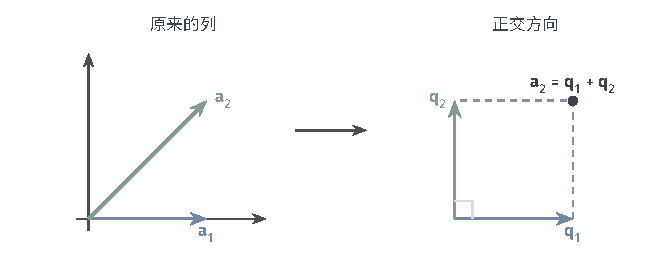
\includegraphics[width=112mm]{figures/00-shared/mathematical-preliminaries-upper/02-linear-spaces/tikz/comprehension-additions/linear-qr-columns.pdf}
  \caption{QR分解把列的方向和组合系数分开。取$\bm a_1=(1,0)^\top$、$\bm a_2=(1,1)^\top$，
  正交化得到$\bm q_1=(1,0)^\top$、$\bm q_2=(0,1)^\top$，并有$\bm a_1=\bm q_1$、
  $\bm a_2=\bm q_1+\bm q_2$，故$\bm R=\left[\begin{smallmatrix}1&1\\0&1\end{smallmatrix}\right]$。
  虚线补出第二列的分量。}
  \label{fig:vol1-add-linear-qr-columns}
\end{figure}

这一分解的用处在于，涉及列空间的计算可以改在标准正交的$\bm Q$上进行，坐标由内积直接读出，不必再解Gram方程。第~\ref{chap:linear-equations-and-optimization}章解方程与最小二乘问题时就是这样使用它的。

\subsubsection{列相关时的处理}

定理~\ref{thm:ls-gram-schmidt}要求各列线性无关。若不满足，某一步会出现$\bm u_j=\bm0$。由正交分解，这恰好说明$\bm a_j$已在前面方向张成的空间中，没有带来新方向。这时不能对零向量归一化，应跳过这一列，只在$\bm R$中记下它的系数$\langle\bm a_j,\bm q_i\rangle$。跳过它不影响后续各列，因为张成的空间没有变。

全部处理完以后，留下的$\bm q$的个数等于列空间的维数$r=\operatorname{rank}\bm A$，仍有$\bm A=\bm Q\bm R$。其中$\bm Q\in\mathbb R^{m\times r}$的列是列空间的标准正交基；$\bm R\in\mathbb R^{r\times d}$各行从左到右第一个非零元的位置逐行右移。$r<d$时$\bm R$不是方阵，不能求逆。下面是最小的例子。
\begin{example}[列相关时跳过零余量]
\label{ex:ls-qr-dependent-columns}
给定：$\bm A=[\bm a_1\ \bm a_2]$，$\bm a_1=(1,0)^\top$、$\bm a_2=(2,0)^\top$。

计算：$\bm q_1=\bm a_1$。$\langle\bm a_2,\bm q_1\rangle=2$，扣除后$\bm u_2=\bm a_2-2\bm q_1=\bm0$，所以跳过$\bm a_2$，只在$\bm R$中记下系数$2$。于是$r=1$，
\[
\begin{gathered}
\bm Q=\begin{bmatrix}1\\0\end{bmatrix},\\
\bm R=\begin{bmatrix}1&2\end{bmatrix},\\
\bm Q\bm R=\begin{bmatrix}1&2\\0&0\end{bmatrix}=\bm A .
\end{gathered}
\]

结论：列空间仍是$x$轴，$\bm Q$的一列构成它的标准正交基，$\operatorname{rank}\bm A=1$。
\end{example}
于是在精确算术下，同一过程也给出列空间的一组标准正交基与矩阵的秩。有限精度下，扣除后的余量很少恰好为零；怎样判断它“算作零”，以及怎样改写扣除顺序以减少正交性的损失，属于数值计算问题，在第~\ref{sec:ls-numerical-sensitivity}节讨论。

\subsection{正交投影}
\label{sec:ls-orthogonal-projection}

标准正交基使子空间中的分量可以逐个读出。把这些分量合在一起，就得到正交投影。本小节证明它是子空间中离原向量最近的点，再把它写成矩阵，并给出判断一个矩阵是否为正交投影的方法。

\paragraph{向子空间的正交分解}
若$\bm q_1,\ldots,\bm q_r$是子空间$U$的标准正交基，引理~\ref{lem:ls-orthogonal-decomposition}中的Gram矩阵是单位矩阵，Gram方程直接给出$\bm a=(\langle\bm q_i,\bm x\rangle)_i$。于是分解可以直接写出：
\begin{equation}
 \bm x=\underbrace{\sum_{j=1}^r\langle\bm x,\bm q_j\rangle\bm q_j}_{\bm u\in U}+\underbrace{\Bigl(\bm x-\sum_{j=1}^r\langle\bm x,\bm q_j\rangle\bm q_j\Bigr)}_{\bm r\in U^\perp}.
 \label{eq:ls-orthonormal-projection}
\end{equation}
$\bm u$称为$\bm x$在$U$上的正交投影。$\bm u$与$\bm r$正交，由勾股定理，
\[
 \lVert\bm x\rVert^2=\lVert\bm u\rVert^2+\lVert\bm r\rVert^2\geq\sum_{j=1}^r\langle\bm x,\bm q_j\rangle^2.
\]
即沿一部分标准正交方向读出的系数，其平方和不超过总长度的平方；等号恰在$\bm x\in U$时成立。

现在证明$\bm u$是最近点。对任意$\bm v\in U$，$\bm x-\bm v=(\bm x-\bm u)+(\bm u-\bm v)$的两项分别属于$U^\perp$和$U$。由勾股定理，
\[
 \lVert\bm x-\bm v\rVert^2=\lVert\bm x-\bm u\rVert^2+\lVert\bm u-\bm v\rVert^2\geq\lVert\bm x-\bm u\rVert^2.
\]
等号只在$\bm v=\bm u$时成立，所以$\bm u$是唯一的最近点。基不是标准正交时，同样可以先解Gram方程求出投影；实际求解时不必显式形成逆矩阵。

最近点的唯一性来自内积确定的正交分解。第~\ref{sec:ls-quotient-norms}节已经证明一般范数下最近点存在，示例~\ref{ex:ls-linf-nonunique-nearest}却在$\ell_\infty$范数下给出了无穷多个最近点；同一个点在欧氏范数下的最近点只有原点，因为$\lVert\bm y-(t,0)^\top\rVert_2^2=t^2+1$只在$t=0$时取最小值。

下面用标准正交基重算前面的正交分解。
\begin{example}[用标准正交基重算正交分解]
\label{ex:ls-orthonormal-projection-line}
给定：$U=\operatorname{span}\{\bm q_1\}$，$\bm q_1=(1,1,1)^\top/\sqrt3$，$\bm y=(1,1.1,0.9)^\top$。

计算：$\langle\bm y,\bm q_1\rangle=3/\sqrt3=\sqrt3$，投影为$\sqrt3\,\bm q_1=(1,1,1)^\top$，余量为$(0,0.1,-0.1)^\top$，它与$\bm q_1$正交。

结论：结果与示例~\ref{ex:ls-orthogonal-decomposition-line}相同，但这里不需要解Gram方程。
\end{example}

\paragraph{投影矩阵}
\label{sec:ls-projection-matrices}
正交投影随原向量线性变化。记$\bm y$在$U$上的正交投影为$\bm p$。$\bm y_1,\bm y_2$的正交分解相加、数乘后仍是正交分解，由分解的唯一性，投影也随之相加、数乘。所以$\bm y\mapsto\bm p$是一个线性映射，称为到$U$的正交投影。

在欧氏内积下，它可以写成矩阵。设$\bm Q$的列是$U$的标准正交基。由$\bm p=\sum_j\langle\bm q_j,\bm y\rangle\bm q_j=\bm Q\bm Q^\top\bm y$，到$U$的正交投影是
\begin{equation}
\begin{gathered}
\bm P_U=\bm Q\bm Q^\top,\\
\bm P_U^\top=\bm P_U,\\
\bm P_U^2=\bm P_U.
\end{gathered}
\label{eq:linear-algebra-orthogonal-projector}
\end{equation}
两条性质都可以直接验证。由$\bm Q^\top\bm Q=\bm I$，$\bm P_U^2=\bm Q(\bm Q^\top\bm Q)\bm Q^\top=\bm Q\bm Q^\top$，即幂等：已经在$U$中的点再投影一次不变。$(\bm Q\bm Q^\top)^\top=\bm Q\bm Q^\top$，即对称：内积中可以把投影移到另一侧。此外$\operatorname{range}\bm P_U=\operatorname{range}\bm Q=U$。$\bm Q$不是方阵时，$\bm P_U$通常不是单位矩阵，它只保留$U$中的分量。

\paragraph{正交投影、斜投影与幂等}
拿到一个矩阵，怎样判断它是不是正交投影？幂等性只说明它是某种投影，不说明它给出最近点。一般的幂等矩阵$\bm P$把$\bm y$分成$\bm P\bm y$与$\bm y-\bm P\bm y$两部分，前者在像中，后者在零空间中，因为$\bm P(\bm y-\bm P\bm y)=\bm P\bm y-\bm P^2\bm y=\bm0$。但两部分不必正交。这种映射称为\term{斜投影}（oblique projection）。

\begin{example}[反例：幂等而不对称的投影]
\label{ex:ls-oblique-projection}
取
\[
 \bm P=\begin{bmatrix}1&-1\\0&0\end{bmatrix}.
\]
直接相乘得$\bm P^2=\bm P$，所以它幂等；它把$(y_1,y_2)^\top$送到$x$轴上的$(y_1-y_2,0)^\top$。残差$\bm y-\bm P\bm y=(y_2,y_2)^\top$与$x$轴方向$(1,0)^\top$的内积是$y_2$，$y_2\neq0$时不为零，所以$\bm P\bm y$不是$x$轴上离$\bm y$最近的点。这个$\bm P$也不对称：$\bm P^\top\neq\bm P$。
\end{example}

对称性正是正交的条件。若$\bm P$幂等且对称，对任意$\bm y,\bm z$有
\[
 (\bm y-\bm P\bm y)^\top\bm P\bm z=\bm y^\top(\bm P-\bm P^\top\bm P)\bm z=\bm y^\top(\bm P-\bm P^2)\bm z=0,
\]
即残差与整个像正交。于是$\bm y=\bm P\bm y+(\bm y-\bm P\bm y)$是$\bm y$关于像空间的正交分解，由分解的唯一性，$\bm P$就是到其像的正交投影。所以判别分两步：先验幂等，判断是不是投影；再验对称，判断是不是正交投影。

\section{线性泛函的内积表示与伴随}
\label{sec:ls-adjoints}

第~\ref{sec:ls-dual-spaces}节的读取规则属于对偶空间，与被读取的向量不在同一个空间；转置在那里是对偶映射的矩阵。有了内积，每个读取都可以写成与一个固定向量的内积，对偶映射也就变成内积空间之间的映射，称为伴随。第~\ref{sec:ls-orthogonality}节证明四个基本子空间的正交关系时，用到的正是伴随在欧氏内积下的形式：内积左侧的$\bm A$可以改写成右侧的$\bm A^\top$。

\subsection{线性泛函的内积表示}
\phantomsection
\label{sec:ls-riesz-representation}
在$\mathbb R^d$的欧氏内积下，加权读取$\varphi(\bm x)=\bm a^\top\bm x$就是与向量$\bm a$的内积。在一般有限维内积空间中，每个读取也都能这样写。
\begin{theorem}[有限维Riesz表示定理]
\label{thm:ls-riesz-representation}
设$V$是有限维内积空间。对每个$\varphi\in V^*$，存在唯一的$\bm v_\varphi\in V$，使$\varphi(\bm x)=\langle\bm x,\bm v_\varphi\rangle$对所有$\bm x\in V$成立。
\end{theorem}
\begin{proof}
取$V$的一组标准正交基$\bm q_1,\ldots,\bm q_d$（第~\ref{sec:ls-orthonormal-basis-construction}节），令$\bm v_\varphi=\sum_j\varphi(\bm q_j)\bm q_j$。由式~\eqref{eq:ls-orthonormal-expansion}，$\bm x=\sum_j\langle\bm x,\bm q_j\rangle\bm q_j$，于是
\[
 \varphi(\bm x)=\sum_j\langle\bm x,\bm q_j\rangle\varphi(\bm q_j)=\Bigl\langle\bm x,\sum_j\varphi(\bm q_j)\bm q_j\Bigr\rangle=\langle\bm x,\bm v_\varphi\rangle.
\]
若$\bm v,\bm v'$都满足要求，则$\langle\bm x,\bm v-\bm v'\rangle=0$对一切$\bm x$成立，取$\bm x=\bm v-\bm v'$得$\bm v=\bm v'$。
\end{proof}
对应$\varphi\mapsto\bm v_\varphi$保持线性组合，这由表示向量的唯一性得到；每个$\bm v$又都表示读取$\langle\cdot,\bm v\rangle$。所以这个对应是$V^*$到$V$的双射。在它之下，标准正交基的对偶基就是这组基本身，因为第$j$个坐标读取是$\bm x\mapsto\langle\bm x,\bm q_j\rangle$。对一般的基，对偶基对应的向量与原基不同：图~\ref{fig:ls-dual-basis-readout}中的红色箭头$\bm b^1,\bm b^2$，正是对偶读取$\varphi_1,\varphi_2$在欧氏内积下对应的向量。

表示向量依赖内积，读取本身却不依赖。在$\mathbb R^d$上取加权内积$\langle\bm x,\bm y\rangle_{\bm M}=\bm x^\top\bm M\bm y$，同一个读取$\varphi(\bm x)=\bm a^\top\bm x=\bm x^\top\bm M(\bm M^{-1}\bm a)$对应的向量是$\bm M^{-1}\bm a$，而不是$\bm a$。函数空间中也是如此。
\begin{example}[积分读取在两点内积下的表示向量]
\label{ex:ls-riesz-integral-two-point}
给定：$P_1$上的内积$\langle f,g\rangle=f(0)g(0)+f(1)g(1)$与读取$\varphi(f)=\int_0^1f(t)\,\mathrm dt$。

计算：对$f=a+bt$，$\varphi(f)=a+b/2$。另一方面，$f$与常数函数$\tfrac12$的内积为
\[
 \Bigl\langle f,\tfrac12\Bigr\rangle=\tfrac12\bigl(f(0)+f(1)\bigr)=\tfrac12(a+a+b)=a+\frac b2 .
\]

结论：$\bm v_\varphi$是常数函数$\tfrac12$。这也说明梯形公式$\tfrac12\bigl(f(0)+f(1)\bigr)$对一次函数精确。
\end{example}
表示向量还给出读取的大小。由Cauchy--Schwarz不等式，$|\varphi(\bm x)|\leq\lVert\bm x\rVert\,\lVert\bm v_\varphi\rVert$；$\bm v_\varphi\neq\bm0$时，取$\bm x=\bm v_\varphi/\lVert\bm v_\varphi\rVert$可取到等号。所以仿照第~\ref{sec:ls-dual-norms}节，在单位球上取读取的最大值，得到
\[
 \lVert\varphi\rVert_*=\max_{\lVert\bm x\rVert\leq1}|\varphi(\bm x)|=\lVert\bm v_\varphi\rVert .
\]
在$\mathbb R^d$的欧氏内积下，这就是$\ell_2$范数的对偶范数仍为$\ell_2$范数。

\subsection{伴随与特殊线性算子}
对偶映射把输出端的读取$f$传回输入端，得到读取$f\circ T$。若把两端的读取都换成表示它的向量，就得到伴随。
\begin{definition}[伴随]
\label{def:linear-algebra-adjoint}
设$T:V\to W$是两个有限维实内积空间之间的线性映射。若存在$T^\star:W\to V$使
\begin{equation}
 \langle T\bm x,\bm y\rangle_W=\langle\bm x,T^\star\bm y\rangle_V
 \label{eq:ls-adjoint-pairing}
\end{equation}
对所有$\bm x\in V$、$\bm y\in W$成立，则$T^\star$称为$T$的\term{伴随}（adjoint）。
\end{definition}

伴随总存在且唯一。固定$\bm y\in W$，$\bm x\mapsto\langle T\bm x,\bm y\rangle_W$是$V$上的线性泛函。由定理~\ref{thm:ls-riesz-representation}，存在唯一的向量使它写成与该向量的内积，把这个向量记为$T^\star\bm y$。$T^\star$对$\bm y$线性：
\[
 \langle\bm x,aT^\star\bm y+bT^\star\bm y'\rangle_V=a\langle T\bm x,\bm y\rangle_W+b\langle T\bm x,\bm y'\rangle_W=\langle T\bm x,a\bm y+b\bm y'\rangle_W,
\]
由表示向量的唯一性，$T^\star(a\bm y+b\bm y')=aT^\star\bm y+bT^\star\bm y'$。

用对偶映射的语言说，把$\bm y\in W$看成读取$\langle\cdot,\bm y\rangle_W$，则$T'$把它送到读取$\langle T\,\cdot,\bm y\rangle_W=\langle\cdot,T^\star\bm y\rangle_V$。所以伴随就是借内积把读取换成向量以后的对偶映射。

具体计算时，取$V,W$的基。由坐标下的内积公式，两边的内积写成$\langle\bm x,\bm x'\rangle_V=\bm x^\top\bm M_V\bm x'$、$\langle\bm y,\bm y'\rangle_W=\bm y^\top\bm M_W\bm y'$，这里$\bm x,\bm y$等指坐标，$\bm M_V,\bm M_W$是两组基的Gram矩阵，对称正定因而可逆。设$T$的矩阵为$\bm A$，伴随的矩阵为$\bm B$。式~\eqref{eq:ls-adjoint-pairing}要求$(\bm A\bm x)^\top\bm M_W\bm y=\bm x^\top\bm M_V\bm B\bm y$对所有$\bm x,\bm y$成立。取$\bm x,\bm y$为标准坐标向量逐个比较元素，这等价于$\bm A^\top\bm M_W=\bm M_V\bm B$，即
\begin{equation}
 \bm B=\bm M_V^{-1}\bm A^\top\bm M_W.
 \label{eq:ls-weighted-adjoint}
\end{equation}
两端都取标准正交基时，$\bm M_V,\bm M_W$都是单位矩阵，伴随矩阵就是$\bm A^\top$，与对偶映射的矩阵相同。一般情形下，伴随既不是单纯转置，也不是转置再求逆。下面的例子说明这一点。
\begin{example}[加权内积下的伴随]
\label{ex:ls-weighted-adjoint}
给定：$V=W=\mathbb R^2$都取加权内积$\langle\bm x,\bm y\rangle_{\bm M}=\bm x^\top\bm M\bm y$，$\bm M=\operatorname{diag}(4,1)$；$T\bm x=\bm A\bm x$，其中
\[
 \bm A=\begin{bmatrix}0&1\\0&0\end{bmatrix}.
\]

计算：由式~\eqref{eq:ls-weighted-adjoint}，
\[
 \bm B=\bm M^{-1}\bm A^\top\bm M
 =\begin{bmatrix}1/4&0\\0&1\end{bmatrix}\begin{bmatrix}0&0\\1&0\end{bmatrix}\begin{bmatrix}4&0\\0&1\end{bmatrix}
 =\begin{bmatrix}0&0\\4&0\end{bmatrix}.
\]
直接核对：$\bm A\bm x=(x_2,0)^\top$，$\langle\bm A\bm x,\bm y\rangle_{\bm M}=4x_2y_1$；$\bm B\bm y=(0,4y_1)^\top$，$\langle\bm x,\bm B\bm y\rangle_{\bm M}=x_2\cdot4y_1$，两者相等。

结论：伴随矩阵是$\bm B$，而不是$\bm A^\top$：
\[
 \bm B=\begin{bmatrix}0&0\\4&0\end{bmatrix}\neq\begin{bmatrix}0&0\\1&0\end{bmatrix}=\bm A^\top.
\]
\end{example}
对偶映射的矩阵总是$\bm A^\top$；伴随与它的差别，来自读取与向量之间的对应$\bm a\mapsto\bm M^{-1}\bm a$随内积改变。四个基本子空间正交关系的证明只用到配对恒等式，所以在一般内积空间中同样有$\ker T^\star=(\operatorname{im}T)^\perp$、$\ker T=(\operatorname{im}T^\star)^\perp$。

\paragraph{伴随的运算规则}
由配对定义可以逐条推出伴随的运算规则：
\[
 \begin{gathered}
(T+S)^\star=T^\star+S^\star,\\
(cT)^\star=c\,T^\star,\\
(TS)^\star=S^\star T^\star,\\
T^{\star\star}=T.
 \end{gathered}
\]
例如$\langle TS\bm x,\bm y\rangle=\langle S\bm x,T^\star\bm y\rangle=\langle\bm x,S^\star T^\star\bm y\rangle$，复合的伴随与乘积的转置一样反转次序；恒等映射的伴随是自身。图~\ref{fig:ls-adjoint-action-transfer}画出伴随怎样把配对从输出端搬回输入端。

伴随不是逆：逆把输出复原成输入，伴随只把作用从内积的一侧移到另一侧。
\begin{example}[反例：伴随不是逆]
\label{ex:ls-adjoint-not-inverse}
给定：非零内积空间$V$上的算子$T=2\operatorname{id}$。

验证：$\langle2\bm x,\bm y\rangle=\langle\bm x,2\bm y\rangle$对一切$\bm x,\bm y$成立，所以$T^\star=2\operatorname{id}$；而$T^{-1}=\tfrac12\operatorname{id}$。

结论：$T^\star\neq T^{-1}$。
\end{example}
\begin{figure}[!htb]
  \centering
  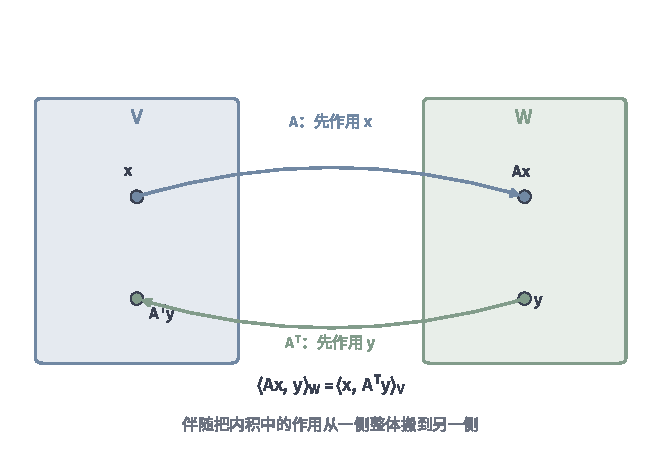
\includegraphics[width=112mm]{figures/00-shared/mathematical-preliminaries-upper/02-linear-spaces/matplotlib/ls-adjoint-action-transfer/ls-adjoint-action-transfer.pdf}
  \caption{内积伴随把输出端的配对搬回输入端。左：$T:V\to W$把$\bm x$映成$T\bm x$，与$\bm y\in W$配对；右：伴随$T^\star:W\to V$把$\bm y$映回$T^\star\bm y\in V$，使$\langle T\bm x,\bm y\rangle_W=\langle\bm x,T^\star\bm y\rangle_V$。标准欧氏内积下$T^\star$就是转置；它反转的是配对的方向，不是逆作用。箭头与空间为解析示意。}
  \label{fig:ls-adjoint-action-transfer}
\end{figure}

\paragraph{自伴、正交与正规算子}
对算子$T:V\to V$，伴随仍是$V$上的算子，可以与$T$比较。若$T^\star=T$，称$T$为\term{自伴}（self-adjoint）算子，它在标准坐标下对应对称矩阵。若$Q^\star Q=\operatorname{id}$，则$Q$保持内积：$\langle Q\bm x,Q\bm y\rangle=\langle\bm x,Q^\star Q\bm y\rangle=\langle\bm x,\bm y\rangle$，称为正交算子。它在标准坐标下对应第~\ref{sec:ls-orthogonal-matrices}节的正交矩阵；由方阵的单侧逆即双侧逆，$Q^{-1}=Q^\star$。满足$TT^\star=T^\star T$的算子称为\term{正规}（normal）算子，自伴算子与正交算子都是正规算子。这些算子的谱性质在第~\ref{chap:linear-analysis}章讨论，这里只给出定义。

\paragraph{复空间中的泛函表示与伴随}
复空间沿用前面“第一变量共轭线性、第二变量线性”的约定。这时线性泛函应写成$\varphi(\bm x)=\langle\bm v,\bm x\rangle$，让$\bm x$处于线性的变量位置。若$\bm q_1,\ldots,\bm q_d$是标准正交基，则$\bm v=\sum_j\overline{\varphi(\bm q_j)}\bm q_j$；代入各基向量即可核对读数。表示向量随泛函作共轭线性变化，这与实空间中的线性对应不同。

例如在$\mathbb C$的标准内积$\langle v,z\rangle=\overline v z$下，泛函$\varphi(z)=(1+\mathrm i)z$对应$v=1-\mathrm i$，因为$\overline v z=(1+\mathrm i)z$。若交换两个变量的位置，得到的表达式关于$z$共轭线性，不再是线性泛函。所以共轭来自内积约定，不能从实数公式中直接删去。

两个复内积空间之间的伴随仍由$\langle T\bm x,\bm y\rangle_W=\langle\bm x,T^\star\bm y\rangle_V$定义。在标准正交基下，若$T$的矩阵为$\bm A$，伴随的矩阵就是$\bm A^*$；若两端基的Gram矩阵为$\bm M_V,\bm M_W$，则为$\bm M_V^{-1}\bm A^*\bm M_W$。这与代数对偶映射的矩阵$\bm A^\top$不同：后者只复合线性泛函，不涉及内积和共轭。复空间中，自伴矩阵满足$\bm A=\bm A^*$；保持内积的方阵满足$\bm A^*\bm A=\bm I$，称为酉矩阵。
